\chapter{Analogiebetrachtungen}
\label{kap:4}
\bookmarksetupnext{level=subsubsection}
\chapterinfo{Auf Grundlage der bereits erarbeiteten Annahmen werden Entsprechungen zum primären Lernbereich in einem sekundären Analogbereich benannt, die objektal umgesetzt und begrifflich-mathematisch mit dem Primärbereich verknüpft werden.}

\textit{Auf Grundlage der bereits erarbeiteten Annahmen werden Entsprechungen zum primären Lernbereich in einem sekundären Analogbereich benannt, die objektal umgesetzt und begrifflich-mathematisch mit dem Primärbereich verknüpft werden.}

\section{Kraftfelder der Analogie}
\label{sec:fields2}
Zur erleichterten Nachvollziehbarkeit der anschließenden Betrachtungen werden zuvorderst die --- für diese Arbeit --- wichtigsten Eigenschaften von \textit{Gravitationsfeldern} und \textit{Strömungsfeldern} umrissen.

\subsection{Gravitationskraft}
\label{sec:gravity}
Nachdem \textsc{Johannes Kepler} (1571--1630), ein protestantischer Theologe, zwischen 1609 und 1619 seine drei Bewegungsgesetze zur Beschreibung \textit{idealisierter Himmelskörper} publiziert hatte, gelang es dem britischen Physiker \textsc{Robert Hooke} (1635--1703) im Jahr 1684, diese Bewegungen in einen Zusammenhang mit der Masse eines Körpers zu bringen.\footfullcite[vgl.][S\,165--166]{Schiller12016} Die Beschleunigung der jeweils angezogenen Masse $m_2$ beträgt
\begin{equation}
\label{eq:gravity1}
\ddot{r}=G\frac{m_1}{r^2}\qquad\text{mit }G=\SI{6.67E-11}{\metre\cubed\per\kilogram\per\second\squared}
\end{equation}  
mit dem \textit{Schwerpunkt-Schwerpunkts-Abstand} $\abs{\boldsymbol{r}}$ und der \textit{Gravitationskonstanten} $G$. Durch Einsetzen der Erdmasse und des Erdradius gelangt man zu der \textit{Erdbeschleunigung} von $g=\SI[fraction-function=\sfrac]{9.81}{\metre\per\second\squared}$. \par
Die \textit{Lageenergie} eines Körpers in einer Höhe $h$ über der Erdoberfläche ist damit 
\begin{equation}
\label{eq:gravity2}
E_\mathrm{pot}=mgh.
\end{equation}
Wird eine schiefe Ebene gemäß Abbildung \ref{fig:rampe1} betrachtet, so ergeben sich mit der nur in $x$-Richtung wirkenden \textit{Haftreibungskraft} $F_\mathrm{HR}$, dem Ebenenwinkel $\alpha$, dem Betrag der Gravitationskraft $F_\mathrm{G}$ und dem Dreh{\-}impuls $L$ folgende Bedingungen für $x$, $y$ und die \textit{Drehimpulsbilanz}:\vspace*{-2.2cm}\footfullcite[vgl.][S.\,135, 169--170]{Greiner2008II}\vspace*{2.2cm}\newpage
\begin{equation}
\begin{alignedat}{2}
\label{eq:gravity3}
& D: F_\mathrm{HR}r=\dot{L}\\
& x: F_\mathrm{G}\sin(\alpha)-F_\mathrm{HR}=&m\dot{x}\\
& y:F_\mathrm{G}\cos(\alpha)- \underbrace{F_{\mathrm{G}_y}}_{F_\mathrm{N}}=& 0
\end{alignedat}
\end{equation}
%% Autor: Björn Ritterbecks 
%% Letzte Aenderung: 15.06.2016 
\thisfloatsetup{%
  capbesidewidth=\marginparwidth}
\begin{figure}[htbp]
\centering
\usetikzlibrary{decorations.pathmorphing}
\pgfplotsset{width=7cm,compat=1.13}
\small
%\sansmath
\begin{tikzpicture}[
	scale=1,
	ka roehre/.style={fill=white,draw=black!80}
]
\begin{scope}[scale=2.0]
%Rampe
\shade[bottom color=mycolor2!50, top color=mycolor2!10] (-2, 0) -- ++ (4,2) -- ++ (0, -0.2) -- ++ (-3.6, -1.8) -- cycle;
\draw[<->,>={latex[length=0pt 3*4,width=0pt 4]},thick, every node/.style={fill=white,midway}] (-2, 0) -- ++ (4,2);
\draw[dashed] (-2, 0) -- ++ (4,0);
% Ball
\shade[ball color=mycolor!25, opacity=1] (0.91, 2.13) circle (0.60);
% Kräfte
   \draw[->,>={Triangle[length=0pt 3*4,width=0pt 4]}, mycolor4, thick]  (0.91,2.13)   -- ++ (-0.52, -0.28);
  \draw[->,>={Triangle[length=0pt 3*4,width=0pt 4]}, mycolor4, thick]  (1.19,1.60)   -- ++ (-0.52, 1.0); 
  \node at (0.90,2.46) {$\boldsymbol{F}_\mathrm{N}$};  
  \draw[->,>={Triangle[length=0pt 3*4,width=0pt 4]}, mycolor4, thick]  (1.19,1.60)   -- ++ (0.39, 0.20); 
   \node at (1.65,1.7) {$\boldsymbol{F}_\mathrm{HR}$}; 
   \draw[->,>={Triangle[length=0pt 3*4,width=0pt 4]}, mycolor4, thick]  (0.91,2.13)   -- ++ (0.0, -1.28);  
   \node at (1.05,0.95) {$\boldsymbol{F}_\mathrm{G}$};
  \draw[dashed, ->,>={Triangle[length=0pt 3*4,width=0pt 4]}, mycolor4, thick]  (0.39,1.85)   -- ++ (0.52, -1.0); 
  \node at (0.5,1.4) {$\boldsymbol{F}_{\mathrm{G}_y}$};   
    \node at (0.4,2.0) {$\boldsymbol{F}_{\mathrm{G}_x}$};
% Radius   
  \draw[-, thick]  (0.91,2.13)   -- ++ (0.28, -0.53); 
   \node at (1.13,1.93) {$\boldsymbol{r}$};  
   % Länge
    \node at (0.0,0.90) {$l$};  
 % Höhe
 \draw[<->,>={latex[length=0pt 3*4,width=0pt 4]},thick, every node/.style={fill=white,midway}]   (1.19,1.60) -- (1.19, 0) node {$h$};
% Winkel   
  \draw[-, thick]  (0.91,1.8) arc (270:296.57:0.33); 
  \node at (0.98,1.9) {$\alpha$};  
    \draw[-, thick]  (-1.5,0) arc (0:26.57:0.5); 
    \node at (-1.7,0.05) {$\alpha$};   
%Achsen    
   \draw[->,>={Triangle[length=0pt 3*4,width=0pt 4]}, thick]  (-1.0,2.4)   -- ++ (0.63, -1.18); 
   \draw[->,>={Triangle[length=0pt 3*4,width=0pt 4]}, thick]  (-0.7,2.3)   -- ++ (-1.17, -0.60);    
  \node at (-1.75,1.85) {$x$}; 
  \node at (-0.33,1.35) {$y$}; 
  \draw[->,>=latex, mycolor4!50!mycolor2, thick]  (1.28,2.74)  arc (60:120:0.70);  
   \node at (0.91,3.0) {$\boldsymbol{\omega}$};
\end{scope}
\end{tikzpicture}
  \caption[Rollende Kugel auf einer schiefen Ebene]{Eine Kugel rollt eine schiefe Ebene herab. Das Koordinatensystem ist um den Winkel $\alpha +\SI{180}{\degree}$ gedreht, um die Bewegungsgleichungen zu simplifizieren. Sofern die Haftreibung $\boldsymbol{F}_\mathrm{HR}$ betragsmäßig geringer als die Hangabtriebskraft $\boldsymbol{F}_{\mathrm{G}_x}$ ist, gleitet die Kugel die schiefe Ebene herunter. Ein Rollen und damit eine Winkelgeschwindigkeit $\boldsymbol{\omega}$ treten auf, wenn die Rollbedingung $\dot{x}=\omega r$ erfüllt ist. Die Reaktionskräfte sind zum besseren Überblick nicht eingezeichnet (eigene Darstellung).}
  \label{fig:rampe1}
  \vspace{-0pt}
\end{figure}
Der Drehimpuls ist das Kreuzprodukt der \textit{Winkelgeschwindigkeit} $\omega$ mit dem \textit{Trägheitsmoment} $J$, welches sich für eine Vollkugel mit der Mittelachse $a$ und dem Radius $r$ zu
\begin{equation}
\begin{alignedat}{2}
\label{eq:gravity4}
J=&\rho \int a^2\mathrm{d}V = \rho \int_{l=0}^{r}\int_{\theta=0}^{\uppi}\int_{\phi=0}^{2\uppi}l^4\sin^3(\theta)\mathrm{d}l\,\mathrm{d\theta}\,\mathrm{d}\phi\\
= &\frac{2}{5}r^2\underbrace{\rho\frac{4}{3}\uppi r^3}_{=\rho V=m}=\frac{2}{5}mr^2
\end{alignedat}
\end{equation}
berechnet. Analog kann über eine dünne Kugelschale integriert werden, um zu zeigen, dass sich bei einer Hohlkugel der Trägheitsmoment $J=\sfrac{2}{3}mr^2$ ergibt. Überdies muss die Rollbedingung $L=J\omega$ erfüllt sein. Setzt man nun $J$ in die erste Zeile von \eqref{eq:gravity3} ein und löst diese nach $F_\mathrm{HR}$ auf, so kann die Haftreibung in der zweiten Zeile eingesetzt werden, um nach elementarer Umformung die Bewegungsgleichung
\begin{equation}
\label{eq:gravity5}
\frac{5}{7}g\sin(\alpha)=\ddot{x}
\end{equation}
aufzustellen. Mit Hilfe der Beschleunigung ergibt sich die Haftreibung zu \begin{equation}
\label{eq:gravity6}
\frac{2}{7}mg\sin(\alpha)=F_\mathrm{HR},
\end{equation}
was unmittelbar zu der $x$-Position in Abhängigkeit von der Zeit führt:
\begin{equation}
\label{eq:gravity7}
x(t) = \frac{5}{14}g\sin(\alpha)t^2
\end{equation}
In obenstehender Gleichung wird die Rollstrecke in Abhängigkeit der mittleren Geschwindigkeit, die auf einer schiefen Ebene  bei einer Startgeschwindigkeit von $\SI[fraction-function=\sfrac]{0}{\metre\per\second}$ nach $t$ Sekunden $\dot{x}\sfrac{t}{2}$ ist, ausgedrückt.
\subsection{Strömungswiderstandskraft}
Der Beschreibung des Strömungsverhaltens von Fluiden haben sich viele Wissenschaftler zwischen dem 17. und 19. Jahrhundert gewidmet. \textsc{Sir Isaac Newton} mathematisierte beispielsweise die \textit{innere Reibung} der nach ihm benannten \textit{Newton'schen Flüssigkeiten} mit einem Gedankenexperiment:\footfullcite[vgl. für die folgenden Ausführungen][S.\,128--132]{Stroppe2008}\par
Eine zwischen zwei Platten eingeschlossene Flüssigkeit, die mit den Wänden über eine Kontaktfläche $A$ in Berührung steht, wird durch die \textit{Adhäsionskraft} über das Verschieben der oberen Platte mit einer Geschwindigkeit $\dot{x}_0$ mitgezogen. Benachbarte Flüssigkeitsschichten in einem Abstand $\Delta h$ werden über die \textit{Viskosität} des zu untersuchenden Fluids ebenfalls in eine Bewegung mit Geschwindigkeit $\dot{x}_1$ versetzt. Somit kann die innere Reibungskraft des Gases bzw. der Flüssigkeit mittels

\begin{equation}
\label{eq:fluid1}
F_\mathrm{R}=\eta A\frac{\mathrm{d}\dot{x}}{\mathrm{d}h}
\end{equation} 
beschrieben werden. Die \textit{dynamische Viskosität} $\eta$ wird in der Einheit $\si{\pascal\second}$ ausgedrückt und ist temperaturabhängig. Sie beträgt beispielsweise bei $\SI{20}{\celsius}$ für Luft $\SI{18.2}{\pascal\second}$. \par
%% Autor: Björn Ritterbecks 
%% Letzte Aenderung: 15.06.2016 
\begin{marginfigure}
\centering
%\sansmath
\begin{tikzpicture}[
	scale=1,
	ka roehre/.style={fill=white,draw=black!80}
]
\begin{scope}[scale=1.5, rotate=90]
%Wände

\draw (-2,1) -- ++ (4, 0);
\shade[right color=halfgray!50, left color=halfgray!10] (-2, 1) rectangle (2, 1.3);
\shade[bottom color=mycolor!25, top color=mycolor!50] (1.5,1) rectangle (-1.5,-1);
\draw (-2,-1) -- ++ (4, 0);
\shade[left color=halfgray!75, right color=halfgray!25] (-2, -1) rectangle (2, -1.3);
%Höhe
 \draw[<->,>={latex[length=0pt 3*4,width=0pt 4]},thick, every node/.style={fill=white,midway}]   (1.8,1) -- ++ (0, -2.0) node {\footnotesize $h$};
   \draw[<->,>={latex[length=0pt 3*4,width=0pt 4]},thick, every node/.style={fill=none,midway}]   (0.375, -0.40) -- ++ (-0.75,0) node [right=0.03] {\footnotesize $\Delta \dot{x}$};
% Delta h
\draw[dashed, thin] (-1.5, 0.25) -- ++ (-0.2, 0);
\draw[dashed, thin] (-1.5, -0.25) -- ++ (-0.2, 0);
\draw[thin] (-1.5, 1) -- ++ (0, -2);
% Delta \dot{x}
\draw[dashed, thin] (0.375, 0.25) -- ++ (0, -0.75);
\draw[dashed, thin] (-0.375, -0.25) -- ++ (0, -0.25);
\draw [<->,>={latex[length=0pt 3*4,width=0pt 4]},thick, every node/.style={fill=white,midway}] (-1.6,0.25) -- ++ (-0,-0.5) node [below=0.05] {\footnotesize $\Delta h$}; 
  \node at (-0.1,1.14) {\footnotesize$\dot{x}_1$};   
% Geschwindigkeiten
\foreach \x in {0,...,7}
        {
            \draw[->,>={Triangle[length=0pt 3*4,width=0pt 4]}, mycolor4!50!mycolor2, thick] ({-1.5,1-\x*0.25}) -- ++ ({3-\x*0.375},0);
        };  
\draw[dashed] (1.5, 1) -- ++ (-3, -2);

\end{scope}
\end{tikzpicture}
  \caption[Herleitung des \textsc{Newton}'schen Reibungsgesetzes]{Herleitung des \textsc{Newton}'schen Reibungsgesetzes: Eine Flüssigkeit ist zwischen zwei Platten eingebettet. Die linke Platte bewegt sich mit der Geschwindigkeit $\dot{x}_1$ und zieht durch die \textsw{Adhäsionskraft} die Flüssgkeit an der Grenzfläche mit, die wiederum benachtbarte Flüssigkeitsschichten mit verringerter Geschwindigkeit $\dot{x}_2$ in Bewegung versetzt (nach \cite[S\,128]{Stroppe2008}).}
  \label{fig:newton1}
  \vspace{-0pt}
\end{marginfigure}
Großen Wert hat das Reibungsgesetz für den laminaren \textit{Volumenstrom} eines Fluides durch ein Rohr mit Radius $r$ und Länge $l$, dessen Verhalten von \textsc{Hagen} und \textsc{Poiseuille} mittels dem Druckgefälle $\Delta \tau$ als
\begin{equation}
\label{eq:fluid2}
I=\frac{V}{t}=\frac{\uppi r^4\Delta \tau}{8\eta l}
\end{equation} 
modelliert wurde. Diese \textit{biquadratische} Abhängigkeit vom Rohrradius führt dazu, dass dünne Kapillargefäße bei geringen Druckunterschieden zwischen zwei Volumina nahezu keinen Volumenstrom zulassen, was unter anderem beim \textit{Parabelspektrographen} von \textsc{Thomson} Anwendung findet (vgl. Abschnitt \ref{sec:2.2} und Abbildung \ref{fig:thoms2}).\par
Durch die Definition einer mittleren Strömungsgeschwindigkeit und gleichsetzen von \eqref{eq:fluid1} und \eqref{eq:fluid2} gelangt man zu der Reibungskraft einer Rohrströmung, welche von \textsc{Sir George Gabriel Stokes} (1819--1903) auf die Umströmung einer Kugel vom Radius $r$ in das \textit{Stokes'sche Reibungsgesetz} übertragen wurde:
\begin{equation}
\label{eq:fluid3}
F_\mathrm{R}=6\uppi \eta r \dot{x}
\end{equation}
Die beschriebenen Gesetzmäßigkeiten gelten gleichwohl nur für ideale, \textit{inkompressible} Fluide. Möchte man den \textit{Strömungswiderstand} für reale Gase in eine Formel betten, so erhält man mit dem \textit{Staudruck} $\tau=\rho\sfrac{\dot{x}^2}{2}$, dem \textit{Widerstandsbeiwert} $c_\mathrm{W}$, sowie der \textit{Projektionsfläche} des umströmten Körpers
\begin{equation}
\label{eq:fluid4}
F_\mathrm{W}=c_\mathrm{W}A_\mathrm{proj}\frac{\rho\dot{x}^2}{2}.
\end{equation} 
Der Widerstandsbeiwert ist bei kompressiblen Fluiden sowohl von der \textit{Reynolds-Zahl} (benannt nach \textsc{Osborne Reynolds} (1842--1912))
\begin{equation}
\label{eq:fluid5}
Re=\frac{\rho l \dot{x}}{\eta}
\end{equation}
als auch wiederholt von der \textit{Anströmgeschwindigkeit} $\dot{x}$ abhängig. Nach \textsc{Stroppe} darf Luft bis zu einer ungefähren Geschwindigkeit von $\dot{x}=\SI[fraction-function=\sfrac]{240}{\metre\per\second}$ als nicht zusammenpressbar genähert werden\footcite[vgl.][S.\,131]{Stroppe2008}, weswegen die Betrachtung der \textit{Mach-Zahl}, d.\,h. des Quotienten von Anströmungsgeschwindigkeit und \textit{Schallgeschwindigkeit} für die weiteren Betrachtungen keine weitere Berücksichtigung findet.\par
Der \textit{Strömungswiderstandskoeffizient} wird zumeist über direkte Messungen von Geschwindigkeit und Widerstandskraft ermittelt. Eine sehr umfangreiche Meta-Analyse von einigen hundert Versuchsreichen führten \textsc{Clift}, \textsc{Grace} und \textsc{Weber} zu einer abschnittsweise definierten Modellierung des Widerstandsbeiwertes einer Kugel in Relation zu der Reynolds-Zahl $R\kern-.04em e$ (vgl. Tabelle \ref{tab:cwwerte}).\vspace*{-2cm}\footfullcite[siehe][S.\,112]{clift2013}\vspace*{2cm}
\vspace*{-0.1cm}  \thisfloatsetup{
  capbesidewidth=\marginparwidth,}

\begin{table}[htbp]
\centering
%\sffamily,
\small
%\sansmath
\arrayrulecolor{white}
\vspace{0.2cm}
  \rowcolors{2}{halfgray!15}{halfgray!5}
 \setlength{\extrarowheight}{.4em}
			\begin{tabularx}{0.99\textwidth}{l*{1}{>{\RaggedRight\arraybackslash}X}}		
\rowcolor{mycolor}\multicolumn{1}{l}{{\color{white}\textbf{Intervall}}}&  \multicolumn{1}{l}{{\color{white}\textbf{$\boldsymbol{c_\mathrm{W}(R\kern-.04em e)}$ [ohne Einheit]}}}\\
$I_0$:\quad $R\kern-.04em e < 0,01$ &  $\frac{3}{16}+\frac{24}{R\kern-.04em e}$\\
$I_1$:\quad $0,01<R\kern-.04em e \leq 20$ &  $\frac{24}{R\kern-.04em e}\left(1+0,1315R\kern-.04em e^{0,82-0,05\log_{10}(R\kern-.04em e)}\right)$\\
$I_2$:\quad $20<R\kern-.04em e \leq 260$ &  $\frac{24}{R\kern-.04em e}\left(1+0,1935R\kern-.04em e^{0,6305}\right)$\\
$I_3$:\quad $260<R\kern-.04em e \leq 1500$ &  $10^{0,0294\ln^2(R\kern-.04em e)-0,4882\ln(R\kern-.04em e)+1,6435}$\\
$I_4$:\quad $1,5\cdot 10^3 <R\kern-.04em e \leq 1,2\cdot 10^4$ &  $10^{0,0086\ln^3(R\kern-.04em e)-0,1753\ln^2(R\kern-.04em e)+1,1000\ln(R\kern-.04em e)-2,4571}$\\
$I_5$:\quad $1,2\cdot 10^4<R\kern-.04em e \leq 4,4\cdot 10^4$ &  $10^{-0,0120\ln^2(R\kern-.04em e)+0,2766\ln(R\kern-.04em e)-1,918}$\\
$I_6$:\quad $4,4\cdot 10^4<R\kern-.04em e \leq 3,4\cdot 10^5$ &  $10^{-0,0292\ln^2(R\kern-.04em e)+0,6866\ln(R\kern-.04em e)-4,3390}$\\
$I_7$:\quad $3,4\cdot 10^5<R\kern-.04em e \leq 4.0\cdot 10^5$ &  $29,78-5,3\log_{10}(R\kern-.04em e)$\\
$I_8$:\quad $4\cdot 10^5<R\kern-.04em e \leq 10^6$ &  $0,1\log_{10}(R\kern-.04em e)-0,49$\\
$I_9$:\quad $ 10^6<R\kern-.04em e$ &  $0,19-8\cdot 10^6\frac{1}{R\kern-.04em e}$\\		  
		\end{tabularx}
		\caption[Widerstandsbeiwerte in Abhängigkeit von der Reynolds-Zahl]{Abschnittsweise definierte Funktion für die Widerstandsbeiwerte einer homogenen Vollkugel in Abhängigkeit von der Reynolds-Zahl nach \cite[S.\,112]{clift2013}. Die Autoren sprechen allerdings nur von \textsw{Empfehlungen}.}
		\label{tab:cwwerte}
\vspace{0.2cm}		
		\end{table}\vspace*{-4cm}
\newpage
\section{Beispiele für Analogversuche}

Aus den verschiedenen Herangehensweisen, einen Analogieversuch zur Massenspektrometrie zu erstellen, wählt diese Arbeit zwei möglichst unterschiedliche Modellversuche als Exempel aus. Hierbei fungiert einmal eine Magnetanordnung, das andere mal ein Gebläse als Analysator.

\subsection{Magnete}

Die Literaturgrundlage der Staatsexamensarbeiten von \textsc{Böhmer} und \textsc{Mais} ist ein Artikel von \textsc{Bühler} und \textsc{Graf} aus der Zeitschrift \textit{Praxis der Naturwissenschaften} zu einem von ihnen weiterentwickelten Modellversuch zur Massenspektrometrie. 

Das Experiment stellt eine \textit{Weiterentwicklung} eines bereits 1970 von der \textsc{Nuffield Foundation} publizierten Versuchs dar,\footfullcite[vgl.][S.\,262--264]{Nuffield1970} bei welchem Kugellager-Kugeln eines Durchmessers zwischen $\SI{11}{\milli\metre}$ und $\SI{4}{\milli\metre}$ eine Glasröhre hinunterrollen und von einem Hufeisenmagneten in viertelkreisförmig angeordnete Auffangbehälter abgelenkt werden. (vgl. Abb. \ref{fig:nuffsaid}).

%% Autor: Björn Ritterbecks 
%% Letzte Aenderung: 15.06.2016 
\thisfloatsetup{%
  capbesidewidth=\marginparwidth}
\begin{figure}[htbp]
\centering
%\sansmath
 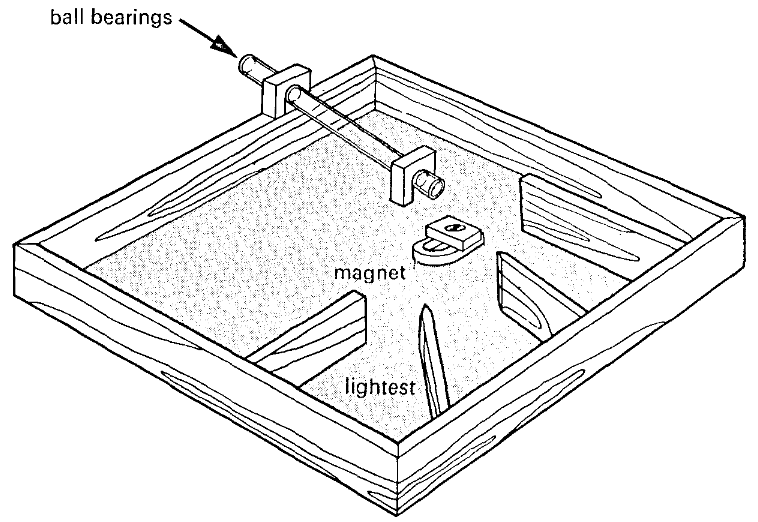
\includegraphics[width=0.99\textwidth]{images/nuffield.png}
  \caption[Funktionsmodell eines Massenspektrometers der Nuffield Foundation]{Funktionsmodell eines Massenspektrometers der Nuffield Foundation. Kugellager-Kugeln rollen durch ein Glasrohr nach unten auf die Platte, wo sie von einem Magneten gestreut werden. Die leichtesten Kugeln werden am Weitesten abgelenkt (entnommen aus \cite[S\,262]{Nuffield1970}).}
  \label{fig:nuffsaid}
  \vspace{-0pt}
\end{figure}

\noindent\textsc{Bühler/Graf}, die bereits im zweiten Satz ihres Artikels \textsc{J. J. Thomson} mit dessen Sohn verwechseln,\footfullcite[vgl.][S.\,33]{Graf2002} befüllen Tischtennisbälle mit Eisenwolle und Nylonwatte, um unterscheidbare Massen-Ladungs-Verhältnisse nachzuahmen.
Der leere Tischtennisball wird durch die Magnetanordnung nicht aus seiner Startrichtung ausgelenkt, der Ball mit $\SI{3}{\gram}$ Eisenwollfüllung wird am Stärksten abgelenkt und der Ball mit jeweils $\SI{3}{\gram}$ Eisenwolle- und Nyolonwattefüllung wird leicht abgelenkt (vgl. Abbildung \ref{fig:graf}).
Sie umreißen ihren Versuch unter anderem mit den Adjektiven \textit{anschaulich}, \textit{objektiv} und \textit{begreifbar}.

%% Autor: Björn Ritterbecks 
%% Letzte Aenderung: 15.06.2016 
\thisfloatsetup{%
  capbesidewidth=\marginparwidth}
\begin{figure}[htbp]
\centering
%\sansmath
 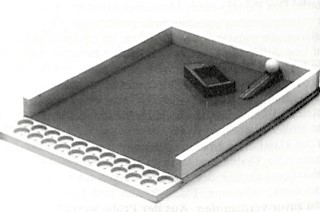
\includegraphics[width=0.99\textwidth]{images/graf.jpg}
  \caption[Funktionsmodell eines Massenspektrometers von Bühler und Graf]{Funktionsmodell eines Massenspektrometers von Bühler und Graf. Tischtennisbälle werden durch eine kleine Bohrung mit Eisenwolle und/oder Nylonwatte befüllt, um Masse-Ladungs-Verhältnisse nachzuahmen (entnommen aus \cite[S\,34]{Graf2002}).}
  \label{fig:graf}
  \vspace{-0pt}
\end{figure}
\noindent Als Motivation für die Neuauflage des Versuches schreiben sie jedoch der Version von 1970 zwei Probleme zu, welche diese gar nicht haben sollte: Sowohl der ">verschiedene Rollwiderstand"<\footcite[vgl.][S.\,35]{Graf2002} als auch das Fehlen der Entmagnetisierung der Kugeln wird moniert, indem auf \textsc{Nuffield} verwiesen wird. Dort heißt es jedoch ">the ball bearings that stick to the magnet will become magnetized and should be dropped several times to demagnetize them."<\footcite[S.\,264]{Nuffield1970} Es wird bei \textsc{Nuffield} mit Kugellagern gearbeitet, die zu den rotationssymmetrischsten und glattesten Kugeln gehören, die man kaufen kann (überdies ist der Rollwiderstand noch von dem Material abhängig, was jedoch bei allen Kugeln \textit{Stahl} ist). Zudem führt das Fallenlassen der Kugeln bereits zu einer Auflösung der \textit{Weiß'schen Bezirke},\footcite[vgl.][S.\,13]{Mais2014} da die Ausrichtung der magnetischen Spins sehr schwach ist.
  \thisfloatsetup{
  capbesidewidth=\marginparwidth,}
\begin{table}[htb]
\centering
%\sffamily,
\small
%\sansmath
\arrayrulecolor{white}
\vspace{0.2cm}
  \rowcolors{2}{halfgray!15}{halfgray!5}
 \setlength{\extrarowheight}{.0em}
			\begin{tabularx}{0.99\textwidth}{l*{1}{>{\RaggedRight\arraybackslash}X}}		
\rowcolor{mycolor}\multicolumn{1}{l}{{\color{white}\textbf{Sektorfeld-Massenspektrometer}}}&  \multicolumn{1}{l}{{\color{white}\textbf{Modellversuch}}}\\
Atome & Acrylkugeln\\
Ionen & mit Eisenwolle gefüllte Kugeln\\
Beschleunigereinheit & Schiefe Ebene\\
Massenanalysator  & Permanentmagnet\\
homogenes Magnetfeld & inhomogenes Magnetfeld\\
Detektor & Röhrensystem\\\bottomrule[5pt]
Elektrisches Feld  & Gravitationsfeld\\
Lorentzkraft $F_\mathrm{L}$& Magnetische Kraft $F_\mathrm{m}$ (sic!)\\
Ionenladung $q$ & Volumen $V_\mathrm{EW}$ der Eisenwolle\\
Elementarladung $e$  & Feste Volumeneinheit $V=\frac{\sfrac{1}{3}\si{\gram}}{\rho_\mathrm{EW}}$\\
Ladung $q=n\cdot e$  & $n\cdot V$\\
		\end{tabularx}
		\caption[Analogien Modellversuch Magnete]{Die Analogie-Zuweisungen nach \textsc{Böhmer} und \textsc{Mais} für den Analogieversuch mit einer Magnetanordnung. Im oberen Teil der Tabelle sind die objektalen, in der unteren Hälfte die begrifflichen Zuordnungen aufgelistet (nach \cite[S.\,16]{Mais2014}).} 
		\label{tab:mais}		
		\end{table}

\noindent Die Hauptprobleme des \textit{Magnetmodells} sind jedoch sowohl die Inhomogenität des magnetischen Feldes, welche eine mathematische Beschreibung der Kugelbewegung nahezu unmöglich macht, als auch die Nichtberücksichtung unterschiedlicher Trägheitsmomente. Bei makroskopischen Modellversuchen können die Kugeln nicht mehr als Punktmassen, was mit den Berechnungen in Abschnitt \ref{sec:fields2} bereits gezeigt wurde, genähert werden. 

Durch \textsc{Böhmer} und \textsc{Mais} wurde dieser Versuch durch eine verbesserte Magnetanordnung und eine bogenförmige Detektoranordnung verbessert. Die abschließenden Analogiebetrachtungen der Examensarbeit von \textsc{Axel Mais} sind in Tabelle \ref{tab:mais} wiedergegeben.


\subsection{Gebläse}

Ein Funktionsmodell zur Massenspektrometrie, welches Gebläse als Analysatoren einsetzt, wurde 1987 im Rahmen einer Zulassungsarbeit von \textsc{Elisabeth Schilling} an der LMU München angefertigt. Der Archivierungszeitraum ist zwar bereits überschritten und damit die Arbeit für alle weiteren Recherchen verloren, jedoch sind die wichtigsten Ergebnisse in einem Artikel der Zeitschrift \textit{der mathematische und naturwissenschaftliche Unterricht} enthalten\footfullcite[vgl.]{Schilling1987}, der dem Verfasser freundlicherweise von Professor Klaus Wendt der Johannes Gutenberg Universität Mainz zugeschickt wurde.

Dieses Funktionsmodell (siehe Abbildung \ref{fig:mnu}) ist die einzig bekannte Ausführung eines geschwindigkeitsfokussierenden Spektrometers. 

Mittels einer $\SI{30}{\centi\metre}$ langen, v-förmigen Rampe, welche eine Steigung von ca. $\SI{20}{\degree}$ besitzt, werden $\SI{20}{\milli\metre}$ große Stahl-, Aluminium- und Plexiglaskugeln beschleunigt. Über eine Platte mit sehr geringer Neigung (ungefähr $1:100$) werden die Kugeln nach ihrer Geschwindigkeit aufgespalten. Je langsamer die Kugel, desto mehr Zeit hat die Erdbeschleunigung, sie abzulenken (vgl. \ref{sec:gravity}). Eine weitere Platte --- diesmal waagerecht montiert --- schließt an die Erste an. An ihrem oberen Ende ist ein Gebläse angebracht, das zu einer Auslenkung der rollenden Kugeln in Abhängigkeit von ihrem Impuls sorgt. Wie mathematisch gezeigt werden kann, kommt es zu einer Fokussierung von Kugeln gleicher Masse und unterschiedlicher Starthöhe. Hierzu sei unter Berücksichtigung der Abschnitte \ref{sec:fields2} und \ref{sec:aston} auf die weitere Analyse in \ref{sec:voraus} verwiesen.

\textsc{Schilling} äußert auch die Gewissheit, dass sich das Funktionsmodell dazu eignet, komplexere Eigenschaften eines Massenspektrometers, wie beispielsweise das Auflösungsvermögen, zu untersuchen.\footcite[vgl.][S.\,37]{Schilling1987}
%% Autor: Björn Ritterbecks 
%% Letzte Aenderung: 15.06.2016 
\thisfloatsetup{%
  capbesidewidth=\marginparwidth,
    capbesideposition=top,
    postcode=flushupp}
\begin{figure*}[htbp]
\centering
%\sansmath
 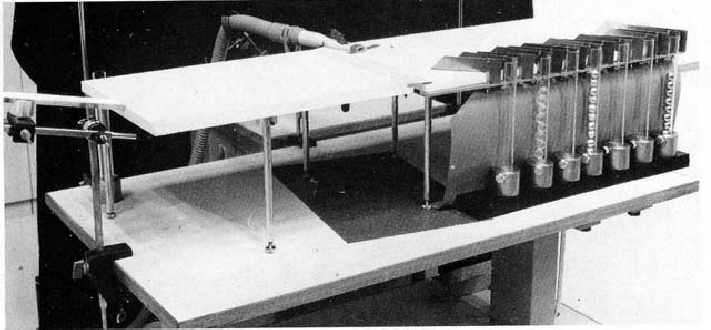
\includegraphics[width=0.99\fulllinewidth]{images/mnu.png}
  \caption[Analogieversuch zu Massenspektrometrie nach \textsc{Luchner}, \textsc{Degner} und \textsc{Schilling} ]{\protect\rule{0cm}{7.6cm}Mechanisches Funktionsmodell eines geschwindigkeitsfokussierenden Massenspektrographen nach \textsc{Schilling} et al.: Kugeln unterscheidbarer Dichte werden die v-förmige Rampe an der linken Seite heruntergerollt, wo sie auf einer schiefen Ebene nach ihrer Geschwindigkeit sortiert werden. Auf der rechten Seite sorgt das Strömungsfeld eines Gebläses für eine Aufspaltung nach den Impulsen (entnommen aus \cite[S\,35]{Schilling1987}).}
  \label{fig:mnu}
  \vspace{-0pt}
\end{figure*}

Abschließend wird anhand von \textit{Stroboskopaufnahmen} --- übrigens ein hervorragendes Mittel zur Visualisierung von Bewegungsprozessen --- eine quantitative Untersuchung der Impulsänderungen $\Delta p$ in Abhängigkeit von der Starthöhe durchgeführt. Hierbei wird ausgenutzt, dass 
\begin{equation}
\begin{alignedat}{2}
\label{eq:impulsaenderung}
\boldsymbol{F}&=m\boldsymbol{\ddot{r}}\\
\Rightarrow \int \boldsymbol{F}\mathrm{d}t &=m\boldsymbol{\dot{r}}=\Delta p
\end{alignedat}
\end{equation} 
gilt, d.\,h. die Krafteinwirkung eines Feldes --- über die Zeit der Einwirkung integriert --- ergibt eine Impulsänderung.

Wenn demnach bekannt ist, wie groß die Krafteinwirkung des Gebläses in Beziehung zu der Entfernung und wie hoch die Geschwindigkeit der sich bewegenden Masse ist, so kann über eine Umformung von \eqref{eq:impulsaenderung} mit der Setzung $\boldsymbol{r}=\boldsymbol{\dot{r}}t$ (vgl. \eqref{eq:bewegung4}) das Integral der Kraft des Strömungsfeldes über dem Abstand von der Mittelachse $x$ berechnet werden, woraus man mittels Division durch die Kugelgeschwindigkeit die Impulsänderung erhält.

\section{Umsetzung}
\label{sec:umsetzung}
Diese Arbeit sollte ursprünglich das Analogiemodell von \textsc{Mais} zu einem Praktikumsversuch weiterentwickeln. Nach einem Hinweis von Frau Professor \textsc{Heidrun Heinke}, dass --- in Anbetracht der Unzulänglichkeiten des Magnetmodells --- auch ein Gebläse als Analysatoreinheit verwendet werden könne, wurde der ursprüngliche Versuchsaufbau nach anfänglichen Testmessungen mit einem handelsüblichen Föhn verworfen (siehe Abschnitt \ref{sec:analysatoren1}).

Aufgrund der Oberflächenähnlichkeit des Funktionsmodells aus \textcite{Schilling1987} mit einem Sektorfeld-Massenspektrometer wird jedoch \textsc{Böhmer} in diesem Punkte gefolgt.\vspace*{-0.4cm}\footcite[vgl. die ausführliche Begründung bei][S.\,26--27]{Boehmer2013}\vspace*{0.4cm} Aus diesem Grund wurde der \textsc{Aston}'sche Massenspektograph als Inkarnation eines EB-Spek{\-}tro{\-}me{\-}ters in Abschn. \ref{sec:aston} auf seine Ablenkung hin untersucht. 

Nach Auswertung der physikalischen Hintergründe wird anhand des zu berücksichtigenden Schemas für wertschöpfende Analogexperimente von \textsc{Kircher} (Tab.\,\ref{tab:ana1}, insbesondere Schritte 3 und 4)  ein Vorschlag die Objektebene betreffend gemacht, welcher zusammengefasst in Tabelle \ref{tab:ana2} zu überblicken ist.

  \thisfloatsetup{
  capbesidewidth=\marginparwidth,}
\begin{table}[htb]
\centering
%\sffamily,
\small
%\sansmath
\arrayrulecolor{white}
\vspace{0.2cm}
  \rowcolors{2}{halfgray!15}{halfgray!5}
 \setlength{\extrarowheight}{.0em}
			\begin{tabularx}{0.99\textwidth}{l*{1}{>{\RaggedRight\arraybackslash}X}}		
\rowcolor{mycolor}\multicolumn{1}{l}{{\color{white}\textbf{Sektorfeld-Massenspektrometer}}}&  \multicolumn{1}{l}{{\color{white}\textbf{Funktionsmodell}}}\\
verschiedene Atome & Kugeln unterscheidbarer Dichte\\
ionisierte Atome & Verschiedene Kugelquerschnittsflächen\\
Hochvakuum & Leerer Experimentiertisch\\
Beschleunigungsspannung & Startrampe mit waagerechtem Auslauf\\
Blendensystem & Schmale Platte lässt nicht alle Geschwindigkeiten zu\\
Analysator I  & Schiefe Ebene\\
Analysator II  & Haartrockner\\
Photoplatte & Auffangbehälter\\
		\end{tabularx}
		\caption[Objektebene der Analogie]{Die Objektebene des Analogieversuches mit einer schiefen Ebene und einem Haartrockner als Massenanalysatoren (eigene Darstellung).} 
		\label{tab:ana2}		
		\end{table}

\noindent Die Anforderungen an die Kugeln sind zwei Gestalt: Erstens muss die Möglichkeit bestehen, verschiedenartige Dichten zu verwenden. Des Weiteren besteht ein Bedarf an einer Projektionsfläche $A_\mathrm{proj}$, welche bestenfalls als Analogon der \textit{Quantelung} von Ladung herhalten kann, indem eine Querschnittsfläche $A_\mathrm{min}$ festgelegt wird, für die weitere Kugelgrößen anhand der Überlegung
\begin{equation}
\label{eq:umsetzung1}
A_i=A_\mathrm{min}\cdot (i+1),\qquad i \in \mathbb{N}\text{ mit }A_i=\uppi r_i^2 
\end{equation} 
festgelegt werden. Dies ist zum Beispiel mit den Radien $r_0=\SI{10}{\milli\metre}$, $r_1=\SI{14}{\milli\metre}$, $r_2=\SI{17}{\milli\metre}$ und $r_3=\SI{20}{\milli\metre}$ erfüllt.

Eine Geschwindigkeitsfokussierung ist nach \ref{sec:aston} nur möglich, wenn die Geschwindigkeiten im Strömungsfeld nicht zu weit auseinander liegen. Wird die Plattengröße klein genug gewählt, so besitzen sämtliche detektierbaren Kugeln gleicher Masse eine Breite $\Delta v$, auf der die Spuren der Kugeln sich nahezu schneiden.

Durch die Auswertung der ersten Messung mit einem Gebläse als Massenanalysator ist augenscheinlich geworden, dass bei den vorhandenen Rampen ca. $\sfrac{1}{4}$ der potentiellen Energie, die durch die Starthöhe vorgegeben wird, nach dem Übergang von Rampe zu Platte nicht in kinetische Energie umgesetzt wird, bzw. dass diese durch ein \textit{Aufprallen} auf der ebenen Fläche verloren geht. Damit ist dieser Energieverlust wesentlich höher als experimentell und theoretisch bestimmte Luftreibungs- und Rollreibungsverluste (ausführlicher inklusive Messdaten siehe Kapitel \ref{kap:5}).

Über einen Vergleich der theoretischen Abschnitte \ref{sec:force1} und \ref{sec:fields2} kann die schiefe Ebene als erster Teil der Massenanalyse eins zu eins auf das elektrische Feld übertragen werden, da Coulombkraft und Gravitationskraft jeweils zu einer Beschleunigung führen, die mit dem Abstand $s$\footnote{Im Folgenden gilt $a \mathop{\hat{=}} $ \textsw{Beschleunigung}, $v \mathop{\hat{=}} $ \textsw{Geschwindigkeit} und $s \mathop{\hat{=}} $ \textsw{Abstand}, um keine doppelte Variablenbelegung zu haben.} zum Quadrat abnimmt, linear mit einem Faktor ($\epsilon_0$ und $G$) skaliert und sich die Masse $m$ des Gravitationspotentials mit der Ladung $q$ des Coulompotentials ersetzen lässt.

Über den zweiten Teil des Analysators sind nur die Erkenntnisse von \textcite{Schilling1987} bekannt. Daher folgt an dieser Stelle die Untersuchung des Haartrockners. In Tabelle \ref{tab:ana3} werden die Ergebnisse jedoch der Übersichtlichkeit halber bereits mit aufgeführt.

  \thisfloatsetup{
  capbesidewidth=\marginparwidth,}
\begin{table}[htb]
\centering
%\sffamily,
\small
%\sansmath
\arrayrulecolor{white}
\vspace{0.2cm}
  \rowcolors{2}{halfgray!15}{halfgray!5}
 \setlength{\extrarowheight}{.40em}
			\begin{tabularx}{0.99\textwidth}{X*{1}{>{\RaggedRight\arraybackslash}X}}		
\rowcolor{mycolor}\multicolumn{1}{l}{{\color{white}\textbf{Sektorfeld-Massenspektrometer}}}&  \multicolumn{1}{l}{{\color{white}\textbf{Funktionsmodell}}}\\
Coulomb-Potential $\phi_\mathrm{Coul} =\frac{1}{4\uppi\epsilon_0}\frac{Q}{r}$ & Gravitationspotential $\phi_\mathrm{Grav}=-G\frac{m}{r}$\\
Elementarladung $q$ & Projektionsfläche $A_\mathrm{min}=\uppi r_\mathrm{min}^2$\\
Gesamtladung $Q=n\cdot q$ & Projektionsfläche $A_i=i\cdot A_\mathrm{min}$\\ 
Potentielle Energie $qU_\mathrm{B}$& Potentielle Energie $mgh$\\
Kinetische Energie $\frac{1}{2}mv^2$& Kinetische Energie $\frac{7}{10}mv^2$\\
Lorentzkraft $F_\mathrm{L}=qvB$ & Strömungswiderstandskraft $F_\mathrm{W}=c_\mathrm{W}A\frac{\rho v^2}{2}$\\
Anzahl detektierter Impulse für $\sfrac{m}{q}=j$ & Aufgefangene Kugeln in Detektor $j$\\
		\end{tabularx}
		\caption[Begriffsebene der Analogie]{Übersicht der begrifflichen Analogien zwischen dem Primär- und Sekundärbereich bei Nutzung einer schiefen Ebene und eines Föhns als Massenanalysatoren. Da bei dem Vergleich zwischen den Lernbereichen der Radius $r$ auftaucht, wird ab dieser Stelle für die Geschwindigkeit $v$ verwendet (eigene Darstellung).} 
		\label{tab:ana3}		
		\end{table}

\section{Gebläse}
\label{sec:analysatoren1}

Obwohl die Überprüfung der erarbeiteten Analogie-Setzungen erst in Kapitel \ref{kap:5} durchgeführt werden wird, muss zuvorderst der gewählte Analysator in Form eines durch einen Föhn hervorgerufenen Strömungsfeldes überprüft werden. Die Messergebnisse werden anschließend mit den abschließenden Werten von \textcite[S.\,53--66]{Mais2014} verglichen.

Hierbei wird auch die Forderung nach einem \textit{gebogenen} Detektor umgesetzt, da die Aufspaltung der Kugeln als Winkelstreuung mit einem festen Mittelpunkt bei $(x, y)\tran$ = $(x, y)\tran (F_\mathrm{max})$, d.\,h. im Punkte der maximalen Krafteinwirkung, gesehen werden kann.

%% Autor: Björn Ritterbecks 
%% Letzte Aenderung: 15.06.2016 
\thisfloatsetup{%
  capbesidewidth=\marginparwidth}
\begin{figure}[htb!p]
\centering
%\sansmath
 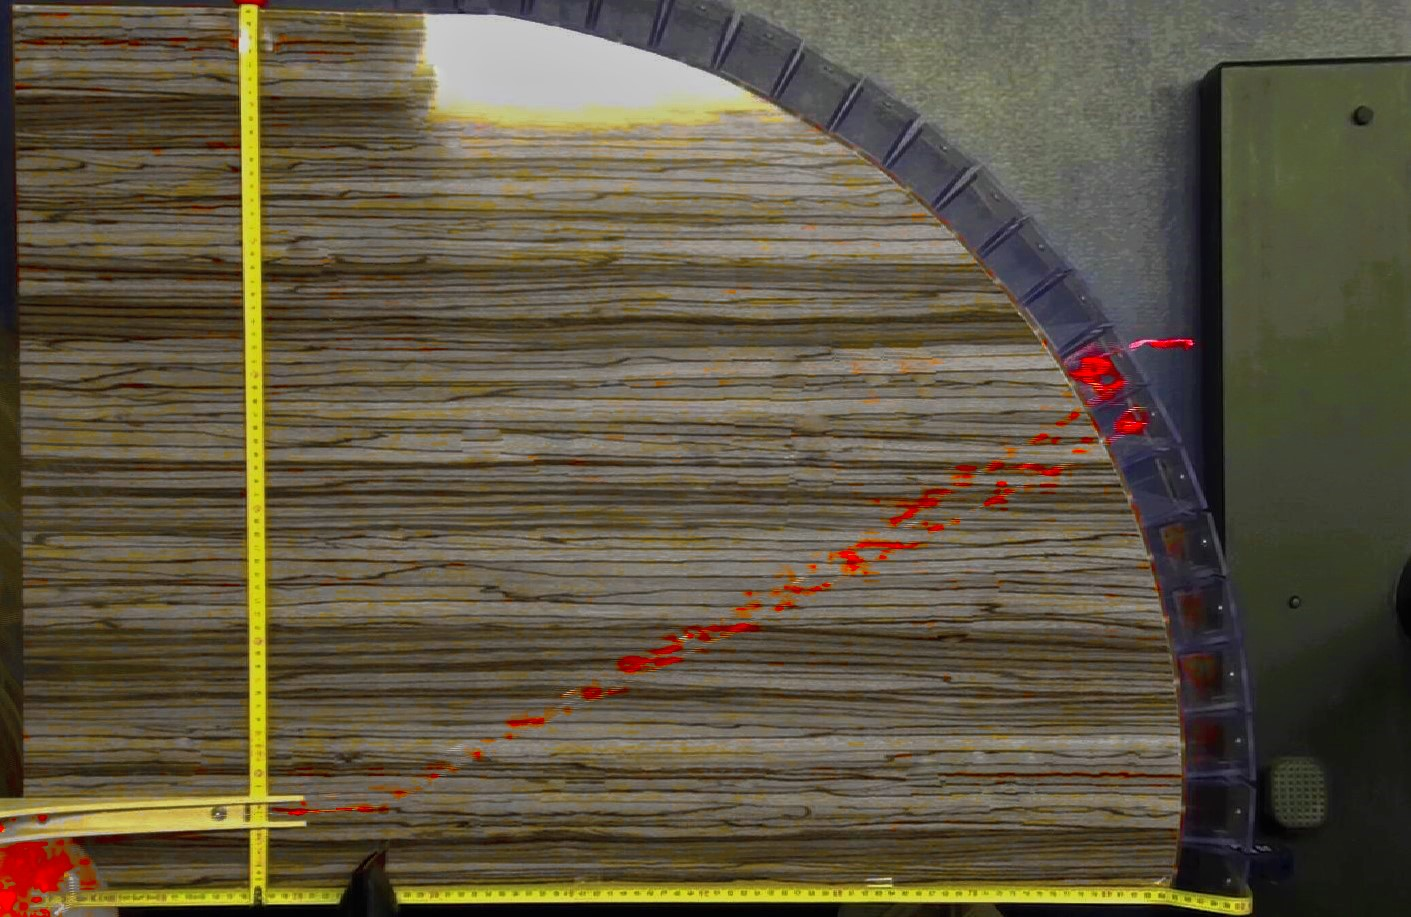
\includegraphics[width=0.99\textwidth]{images/strobe1.jpg}
  \caption[Exemplarische Stroboskopaufnahme der ersten Messreihe]{Exemplarisches Bildschirmfoto mit Stroboskopfilter der ersten Messreihe. Wegen des geringen Kontrastes zwischen den roten Kugeln und der bräunlichen Arbeitsplatte werden Farbfilter angewendet, um die Bahnkurven besser erkennbar zu machen. Bei der Auswertung einzelner Bilder in der Software \textit{Tracker} sind die Kugeln bis auf eine Bewegungsverzerrung gut erkennbar.}
  \label{fig:strobe1}
  \vspace{-0pt}
\end{figure}

Abbildung \ref{fig:strobe1} zeigt den rudimentären Versuchsaufbau nebst der stoboskopischen Aufnahme zweier Kugelbahnen. Ein im Baumarkt erhältliches Reststück einer Arbeitsplatte von etwa $\SI{1.2}{\metre}$ mal $\SI{0.8}{\metre}$ wurde bogenförmig ausgesägt, wobei der Ablenkwinkel von $\SI{0}{\degree}$ auf einer Achse mit der Startrampe liegt. Im Zuge dieser Videoauswertung wird auch die Güte der Rampe untersucht. Diese besitzt eine durch das bloße Auge zu erkennende Asymmetrie, welche den abrollenden Kugeln eine Rotation in $y$-Richtung mitgibt (das im Bildschirmfoto obere Segment der Startvorrichtung ist kürzer als das untere).

Vor den eigentlichen Auswertungen muss daher erstmal ohne angeschalteten Föhn die \textit{Nulllinie} bestimmt werden. Hierzu werden die $10$ von \textcite[S.\,34]{Mais2014} präparierten Kugeln jeweils fünf mal von dem Anschlag bei einer Starthöhe von $h=\SI{55}{\milli\metre}$ abgerollt. Für sämtliche Videoauswertungen wird auf die in der Software \textit{Tracker} bestimmten Koordinaten eine Unsicherheit von $\SI{0.5}{\centi\metre}$ in beide Richtungen angenommen.

Aufgrund der großen Datenmenge werden an dieser Stelle nur die Bewegungen der ersten Kugel tabellarisch und als Diagramm dargestellt. Bei den weiteren Videoauswertungen wird nur noch die Detektionshäufigkeit in Behälter $i$ betrachtet (siehe Tabelle \ref{tab:nullpunkt1}). 

Es ist auch von Interesse, ob sich die Kugeln hinter der Stelle der Krafteinwirkung auf einer Geraden bewegen, d.\,h. ob die Platte trotz der Ungenauigkeit von Wasserwaagen horizontal ausgerichtet ist. Dazu eignet sich der \textit{Bravais-Pearson-Korrelationskoeffizient}, der genau dann einen der Werte $\pm 1$ annimmt, wenn sich die Messdaten auf einer Geraden mit positiver/negativer Steigung befinden.\footfullcite[vgl.][S.\,111]{Cramer2008} Der B-P-Koeffizient ist über den Quotienten der \textit{empirischen Kovarianz} $s_{xy}$ durch das Produkt der Standardabweichungen $s_x$, $s_y$ (oder \textit{empirische Varianzen}) definiert:
\begin{equation}
\label{eq:b-p-k}
r_{xy}=\frac{s_{xy}}{s_xs_y}=\frac{\sum\limits_{i=1}^{n}(x_i-\overline{x})(y_i-\overline{y})}{\sqrt{\sum\limits_{i=1}^{n}(x_i-\overline{x}^2)}\sqrt{\sum\limits_{i=1}^{n}(y_i-\overline{y})^2}}\\
\end{equation}

  \thisfloatsetup{
  capbesidewidth=\marginparwidth,
}
\begin{table}[!p]
\centering
%\sffamily,
\small
%\sansmath
\arrayrulecolor{white}
\setlength{\arrayrulewidth}{2pt}
\vspace{0.2cm}
  \rowcolors{2}{halfgray!15}{halfgray!5}
 \setlength{\extrarowheight}{.00em}\subfloat{
			\begin{tabularx}{0.99\fulllinewidth}{X*{6}{>{\RaggedLeft\arraybackslash}X}}		
\rowcolor{mycolor} &  \multicolumn{2}{|c}{{\color{white}\textbf{Bahn 1}}} &  \multicolumn{2}{|c}{{\color{white}\textbf{Bahn 2}}}&\multicolumn{2}{|c}{{\color{white}\textbf{Bahn 3}}}\\
\rowcolor{mycolor} \multirow{-2}{*}{{\color{white}\textbf{$\boldsymbol{t}$ in $\boldsymbol{\si{\second}}$}}}& \multicolumn{1}{|r}{{\color{white}\textbf{$\boldsymbol{x}$ in $\boldsymbol{\si{\milli\metre}}$}}}&  \multicolumn{1}{r}{{\color{white}\textbf{$\boldsymbol{y}$ in $\boldsymbol{\si{\milli\metre}}$}}} & \multicolumn{1}{|r}{{\color{white}\textbf{$\boldsymbol{x}$ in $\boldsymbol{\si{\milli\metre}}$}}}&  \multicolumn{1}{r}{{\color{white}\textbf{$\boldsymbol{y}$ in $\boldsymbol{\si{\milli\metre}}$}}}&\multicolumn{1}{|r}{{\color{white}\textbf{$\boldsymbol{x}$ in $\boldsymbol{\si{\milli\metre}}$}}}&  \multicolumn{1}{r}{{\color{white}\textbf{$\boldsymbol{y}$ in $\boldsymbol{\si{\milli\metre}}$}}}\\
0,00	& \multicolumn{1}{|r}{	-53	$\pm$ 5	}&	-1	$ \pm$ 5	 & \multicolumn{1}{|r}{	-68	$ \pm$ 5	}&	-7	$ \pm$ 5	 & \multicolumn{1}{|r}{	-49	$ \pm$ 5	}&	-5	$ \pm$ 5	\\
0,04	& \multicolumn{1}{|r}{	-24	$\pm$ 5	}&	-2	$ \pm$ 5	 & \multicolumn{1}{|r}{	-35	$ \pm$ 5	}&	-5	$ \pm$ 5	 & \multicolumn{1}{|r}{	-17	$ \pm$ 5	}&	-4	$ \pm$ 5	\\
0,08	& \multicolumn{1}{|r}{	14	$\pm$ 5	}&	1	$ \pm$ 5	 & \multicolumn{1}{|r}{	-1	$ \pm$ 5	}&	-2	$ \pm$ 5	 & \multicolumn{1}{|r}{	14	$ \pm$ 5	}&	-5	$ \pm$ 5	\\
0,12	& \multicolumn{1}{|r}{	40	$\pm$ 5	}&	2	$ \pm$ 5	 & \multicolumn{1}{|r}{	29	$ \pm$ 5	}&	-1	$ \pm$ 5	 & \multicolumn{1}{|r}{	61	$ \pm$ 5	}&	-2	$ \pm$ 5	\\
0,16	& \multicolumn{1}{|r}{	68	$\pm$ 5	}&	4	$ \pm$ 5	 & \multicolumn{1}{|r}{	50	$ \pm$ 5	}&	-1	$ \pm$ 5	 & \multicolumn{1}{|r}{	70	$ \pm$ 5	}&	-2	$ \pm$ 5	\\
0,20	& \multicolumn{1}{|r}{	101	$\pm$ 5	}&	8	$ \pm$ 5	 & \multicolumn{1}{|r}{	83	$ \pm$ 5	}&	0	$ \pm$ 5	 & \multicolumn{1}{|r}{	101	$ \pm$ 5	}&	0	$ \pm$ 5	\\
0,24	& \multicolumn{1}{|r}{	131	$\pm$ 5	}&	8	$ \pm$ 5	 & \multicolumn{1}{|r}{	120	$ \pm$ 5	}&	2	$ \pm$ 5	 & \multicolumn{1}{|r}{	132	$ \pm$ 5	}&	2	$ \pm$ 5	\\
0,28	& \multicolumn{1}{|r}{	154	$\pm$ 5	}&	10	$ \pm$ 5	 & \multicolumn{1}{|r}{	143	$ \pm$ 5	}&	4	$ \pm$ 5	 & \multicolumn{1}{|r}{	162	$ \pm$ 5	}&	5	$ \pm$ 5	\\
0,32	& \multicolumn{1}{|r}{	186	$\pm$ 5	}&	13	$ \pm$ 5	 & \multicolumn{1}{|r}{	169	$ \pm$ 5	}&	7	$ \pm$ 5	 & \multicolumn{1}{|r}{	193	$ \pm$ 5	}&	6	$ \pm$ 5	\\
0,36	& \multicolumn{1}{|r}{	216	$\pm$ 5	}&	16	$ \pm$ 5	 & \multicolumn{1}{|r}{	203	$ \pm$ 5	}&	8	$ \pm$ 5	 & \multicolumn{1}{|r}{	222	$ \pm$ 5	}&	10	$ \pm$ 5	\\
0,40	& \multicolumn{1}{|r}{	246	$\pm$ 5	}&	17	$ \pm$ 5	 & \multicolumn{1}{|r}{	234	$ \pm$ 5	}&	8	$ \pm$ 5	 & \multicolumn{1}{|r}{	247	$ \pm$ 5	}&	11	$ \pm$ 5	\\
0,44	& \multicolumn{1}{|r}{	276	$\pm$ 5	}&	18	$ \pm$ 5	 & \multicolumn{1}{|r}{	262	$ \pm$ 5	}&	10	$ \pm$ 5	 & \multicolumn{1}{|r}{	283	$ \pm$ 5	}&	12	$ \pm$ 5	\\
0,48	& \multicolumn{1}{|r}{	300	$\pm$ 5	}&	20	$ \pm$ 5	 & \multicolumn{1}{|r}{	292	$ \pm$ 5	}&	12	$ \pm$ 5	 & \multicolumn{1}{|r}{	309	$ \pm$ 5	}&	14	$ \pm$ 5	\\
0,52	& \multicolumn{1}{|r}{	321	$\pm$ 5	}&	19	$ \pm$ 5	 & \multicolumn{1}{|r}{	321	$ \pm$ 5	}&	13	$ \pm$ 5	 & \multicolumn{1}{|r}{	341	$ \pm$ 5	}&	16	$ \pm$ 5	\\
0,56	& \multicolumn{1}{|r}{	354	$\pm$ 5	}&	22	$ \pm$ 5	 & \multicolumn{1}{|r}{	347	$ \pm$ 5	}&	14	$ \pm$ 5	 & \multicolumn{1}{|r}{	366	$ \pm$ 5	}&	19	$ \pm$ 5	\\
0,60	& \multicolumn{1}{|r}{	388	$\pm$ 5	}&	24	$ \pm$ 5	 & \multicolumn{1}{|r}{	381	$ \pm$ 5	}&	14	$ \pm$ 5	 & \multicolumn{1}{|r}{	398	$ \pm$ 5	}&	20	$ \pm$ 5	\\
0,64	& \multicolumn{1}{|r}{	417	$\pm$ 5	}&	28	$ \pm$ 5	 & \multicolumn{1}{|r}{	411	$ \pm$ 5	}&	16	$ \pm$ 5	 & \multicolumn{1}{|r}{	429	$ \pm$ 5	}&	25	$ \pm$ 5	\\
0,68	& \multicolumn{1}{|r}{	444	$\pm$ 5	}&	28	$ \pm$ 5	 & \multicolumn{1}{|r}{	436	$ \pm$ 5	}&	18	$ \pm$ 5	 & \multicolumn{1}{|r}{	458	$ \pm$ 5	}&	31	$ \pm$ 5	\\
0,72	& \multicolumn{1}{|r}{	479	$\pm$ 5	}&	25	$ \pm$ 5	 & \multicolumn{1}{|r}{	464	$ \pm$ 5	}&	22	$ \pm$ 5	 & \multicolumn{1}{|r}{	483	$ \pm$ 5	}&	31	$ \pm$ 5	\\
0,76	& \multicolumn{1}{|r}{	499	$\pm$ 5	}&	31	$ \pm$ 5	 & \multicolumn{1}{|r}{	496	$ \pm$ 5	}&	24	$ \pm$ 5	 & \multicolumn{1}{|r}{	509	$ \pm$ 5	}&	35	$ \pm$ 5	\\
0,80	& \multicolumn{1}{|r}{	529	$\pm$ 5	}&	29	$ \pm$ 5	 & \multicolumn{1}{|r}{	524	$ \pm$ 5	}&	24	$ \pm$ 5	 & \multicolumn{1}{|r}{	541	$ \pm$ 5	}&	40	$ \pm$ 5	\\
		\end{tabularx}}
		\\
		\subfloat{\begin{tabularx}{0.99\textwidth}{X*{4}{>{\RaggedLeft\arraybackslash}X}}		
		\rowcolor{mycolor} &  \multicolumn{2}{|c}{{\color{white}\textbf{Bahn 4}}} &  \multicolumn{2}{|c}{{\color{white}\textbf{Bahn 5}}}\\
		\rowcolor{mycolor} \multirow{-2}{*}{{\color{white}\textbf{$\boldsymbol{t}$ in $\boldsymbol{\si{\second}}$}}}& \multicolumn{1}{|r}{{\color{white}\textbf{$\boldsymbol{x}$ in $\boldsymbol{\si{\milli\metre}}$}}}&  \multicolumn{1}{r}{{\color{white}\textbf{$\boldsymbol{y}$ in $\boldsymbol{\si{\milli\metre}}$}}} & \multicolumn{1}{|r}{{\color{white}\textbf{$\boldsymbol{x}$ in $\boldsymbol{\si{\milli\metre}}$}}}&  \multicolumn{1}{r}{{\color{white}\textbf{$\boldsymbol{y}$ in $\boldsymbol{\si{\milli\metre}}$}}}\\
0,00	& \multicolumn{1}{|r}{	-25	$\pm$ 5	}&	-8	$ \pm$ 5	 & \multicolumn{1}{|r}{	-5	$ \pm$ 5	}&	1	$ \pm$ 5	\\
0,04	& \multicolumn{1}{|r}{	8	$\pm$ 5	}&	-5	$ \pm$ 5	 & \multicolumn{1}{|r}{	26	$ \pm$ 5	}&	6	$ \pm$ 5	\\
0,08	& \multicolumn{1}{|r}{	41	$\pm$ 5	}&	-8	$ \pm$ 5	 & \multicolumn{1}{|r}{	58	$ \pm$ 5	}&	10	$ \pm$ 5	\\
0,12	& \multicolumn{1}{|r}{	72	$\pm$ 5	}&	-5	$ \pm$ 5	 & \multicolumn{1}{|r}{	86	$ \pm$ 5	}&	11	$ \pm$ 5	\\
0,16	& \multicolumn{1}{|r}{	100	$\pm$ 5	}&	-2	$ \pm$ 5	 & \multicolumn{1}{|r}{	117	$ \pm$ 5	}&	12	$ \pm$ 5	\\
0,20	& \multicolumn{1}{|r}{	126	$\pm$ 5	}&	0	$ \pm$ 5	 & \multicolumn{1}{|r}{	147	$ \pm$ 5	}&	12	$ \pm$ 5	\\
0,24	& \multicolumn{1}{|r}{	161	$\pm$ 5	}&	-1	$ \pm$ 5	 & \multicolumn{1}{|r}{	175	$ \pm$ 5	}&	13	$ \pm$ 5	\\
0,28	& \multicolumn{1}{|r}{	185	$\pm$ 5	}&	-2	$ \pm$ 5	 & \multicolumn{1}{|r}{	208	$ \pm$ 5	}&	16	$ \pm$ 5	\\
0,32	& \multicolumn{1}{|r}{	219	$\pm$ 5	}&	2	$ \pm$ 5	 & \multicolumn{1}{|r}{	237	$ \pm$ 5	}&	14	$ \pm$ 5	\\
0,36	& \multicolumn{1}{|r}{	244	$\pm$ 5	}&	4	$ \pm$ 5	 & \multicolumn{1}{|r}{	265	$ \pm$ 5	}&	17	$ \pm$ 5	\\
0,40	& \multicolumn{1}{|r}{	273	$\pm$ 5	}&	5	$ \pm$ 5	 & \multicolumn{1}{|r}{	292	$ \pm$ 5	}&	20	$ \pm$ 5	\\
0,44	& \multicolumn{1}{|r}{	304	$\pm$ 5	}&	8	$ \pm$ 5	 & \multicolumn{1}{|r}{	327	$ \pm$ 5	}&	20	$ \pm$ 5	\\
0,48	& \multicolumn{1}{|r}{	330	$\pm$ 5	}&	10	$ \pm$ 5	 & \multicolumn{1}{|r}{	348	$ \pm$ 5	}&	25	$ \pm$ 5	\\
0,52	& \multicolumn{1}{|r}{	359	$\pm$ 5	}&	12	$ \pm$ 5	 & \multicolumn{1}{|r}{	378	$ \pm$ 5	}&	26	$ \pm$ 5	\\
0,56	& \multicolumn{1}{|r}{	393	$\pm$ 5	}&	13	$ \pm$ 5	 & \multicolumn{1}{|r}{	405	$ \pm$ 5	}&	28	$ \pm$ 5	\\
0,60	& \multicolumn{1}{|r}{	418	$\pm$ 5	}&	14	$ \pm$ 5	 & \multicolumn{1}{|r}{	437	$ \pm$ 5	}&	29	$ \pm$ 5	\\
0,64	& \multicolumn{1}{|r}{	442	$\pm$ 5	}&	17	$ \pm$ 5	 & \multicolumn{1}{|r}{	465	$ \pm$ 5	}&	30	$ \pm$ 5	\\
0,68	& \multicolumn{1}{|r}{	473	$\pm$ 5	}&	19	$ \pm$ 5	 & \multicolumn{1}{|r}{	494	$ \pm$ 5	}&	34	$ \pm$ 5	\\
0,72	& \multicolumn{1}{|r}{	506	$\pm$ 5	}&	23	$ \pm$ 5	 & \multicolumn{1}{|r}{	521	$ \pm$ 5	}&	35	$ \pm$ 5	\\
0,76	& \multicolumn{1}{|r}{	531	$\pm$ 5	}&	24	$ \pm$ 5	 & \multicolumn{1}{|r}{	549	$ \pm$ 5	}&	37	$ \pm$ 5	\\
0,80	& \multicolumn{1}{|r}{	556	$\pm$ 5	}&	26	$ \pm$ 5	 & \multicolumn{1}{|r}{	577	$ \pm$ 5	}&	41	$ \pm$ 5	\\
				\end{tabularx}}
		\caption[Bestimmung des Drehwinkels]{\protect\rule{0cm}{3.0cm}Die fünf Bahnverläufe von Kugel 1 für die Bestimmung des Drehwinkels, der für das Koordinatensystem gewählt werden muss.} 
		\label{tab:nullpunkt1}	
		\end{table} %\vspace*{-5cm}\newpage

\noindent Da die hier gezeigten Datenkolonnen nicht ausufern sollen, wird eine alternative Form von Gleichung \eqref{eq:b-p-k} verwendet, die sich in Tabellenform verkürzt darstellen lässt:
\begin{equation}
\label{eq:b-p-k2}
r_{xy} = \frac{\overline{xy}-\overline{x}\cdot \overline{y}}{\sqrt{(\overline{x^2}-\overline{x}^2)\cdot (\overline{y^2}-\overline{y}^2)}}
\end{equation}

  \thisfloatsetup{
  capbesidewidth=\marginparwidth,
}
\begin{table}[htb]
\centering
%\sffamily,
\small
%\sansmath
\arrayrulecolor{white}
%\setlength{\arrayrulewidth}{2pt}
\vspace{0.2cm}
  \rowcolors{2}{halfgray!15}{halfgray!5}
 \setlength{\extrarowheight}{.00em}
			\begin{tabularx}{0.99\textwidth}{*{6}{>{\RaggedLeft\arraybackslash}X}}	
			\rowcolor{mycolor} && &&&\\	
\rowcolor{mycolor}  \multirow{-2}{*}{{\color{white}\textbf{$\boldsymbol{\bar{x}}$ in $\boldsymbol{\si{\centi\metre}}$}}} &  \multirow{-2}{*}{{\color{white}\textbf{$\boldsymbol{\bar{y}}$ in $\boldsymbol{\si{\centi\metre}}$}}}&\multirow{-2}{*}{{\color{white}\textbf{$\boldsymbol{\overline{x^2}}$ in $\boldsymbol{\si{\centi\metre\squared}}$}}}&\multirow{-2}{*}{{\color{white}\textbf{$\boldsymbol{\overline{y^2}}$ in $\boldsymbol{\si{\centi\metre}}$}}}&\multirow{-2}{*}{{\color{white}\textbf{$\boldsymbol{\overline{xy}}$ in $\boldsymbol{\si{\centi\metre\squared}}$}}} &\multirow{-2}{*}{{\color{white}\textbf{$\boldsymbol{K_\mathrm{B-P}}$}}}\\
28,6	&	1,8	&	1090,3	&	3,99	&	65,68	&	0,98	\\
29,1	&	1,2	&	1100,9	&	1,78	&	43,89	&	0,96	\\
28,6	&	1,3	&	1102,0	&	2,09	&	47,19	&	0,96	\\
29,4	&	0,5	&	1118,4	&	0,51	&	22,66	&	0,98	\\
28,5	&	1,4	&	1070,7	&	2,80	&	54,25	&	0,99	\\
		\end{tabularx}
		\caption[Überprüfung auf lineare Bewegung]{Überprüfung der Kugelspuren auf Linearität mittels des Bravais-Pearson-Korrelationskoeffizienten} 
		\label{tab:bpk}	
		\end{table} %\vspace*{-5cm}\newpage

\noindent Es ergeben sich die Korrelationskoeffizienten in Tabelle \ref{tab:bpk}, wobei auf eine Angabe der Unsicherheiten auf die Mittelwerte verzichtet wird, da die Koeffizienten rein qualitativ lineares Verhalten angeben sollen und nicht als \textit{Bestimmtheitsmaß} einer linearen \textit{Regression} gebraucht werden. Mit den Korrelationskoeffizienten ist eine geradlinige Bewegung verifiziert, was eine Winkeltransformation, d.\,h. eine Drehung des Koordinatensystems um den mittleren Auslenkwinkel $\phi$ erlaubt.

Mit dem \textit{Arkustangens} der Steigung $\sfrac{\Delta y}{\Delta x}$ lässt sich für jede der $50$ verfolgten Kugeln ein Ablenkwinkel berechnen. Der Mittelwert dieser Winkel ist
\begin{equation}
\label{eq:phi}
\phi = (2,45\pm 0,29)\si{\degree},
\end{equation}
die Unsicherheit berechnet sich hierbei als Wurzel der empirischen Varianz. Diese fünf Kugelspuren sind wie gemessen im Diagramm \ref{fig:trans} und transformiert als \ref{fig:trans2} zu sehen, wobei die Drehung sich aus
\begin{equation}
\begin{alignedat}{2}
x_i^*&=x_i\cdot \cos(\phi)+y_i\cdot \sin(\phi)\text{ und}\\
y_i^*&=-x_i\cdot \sin(\phi)+y_i\cdot \cos(\phi)
\end{alignedat}
\end{equation}
ergibt.

  \thisfloatsetup{%
  capbesidewidth=\marginparwidth}

\begin{figure}[htb!p]
\centering
%\sansmath
\begin{tikzpicture}
\begin{axis}[	
	clip mode=individual, % Verhindet weiße Punkte bei vielfach geplotteten x-Werten
	ymajorgrids,
    xmajorgrids,
          axis x line*=middle,
          axis y line*=center,
    grid style={white,thick},
%	axis on top,
    width=12cm,
    height=8.797cm,
    xmin=-0.1,
    xmax=0.6,
    ymin=-0.025,
    ymax=0.05,
    %/tikz/ybar interval,
    tick align=center,
    xtick align=outside,
    xlabel={$x$},
    ylabel={$y$},   
   x label style={at={(axis cs:0.5,-0.010)}},
    y label style={at={(axis cs:-0.105,0.025)}},
    axis line style={Honeydew4!70!black},
    ticklabel style={Honeydew4!70!black, inner sep=1pt,
                font=\footnotesize},
    yticklabels={  -25, 0,  {$\SI{E-3}{\metre}$}, 50},            
    ytick={  -0.025, 0, 0.025, 0.050, 0.100},
    xtick={-0.1,0,0.1,0.2,0.3,0.4,0.5, 0.6}, 
    xticklabels={-0.1,0,0.1,0.2,0.3,0.4,{$\si{\metre}$}, 0.6},
    scaled ticks=false,
    width=\textwidth,                                   
    label style={font=\small,Honeydew4!70!black,},
    enlarge x limits=true,
    %tick style={draw=none},
    x tick label as interval=false,
       legend style ={ at={(axis cs:0.05,0.05)}, 
            anchor=north west, draw=none, 
            fill=none,align=left, text=Honeydew4!70!black, font=\footnotesize},
        cycle list name=mycolor white,
        smooth
    %nodes near coords={\pgfmathfloatifflags{\pgfplotspointmeta}{0}{}{\pgfmathprintnumber{\pgfplotspointmeta}}},
    %every node near coord/.append style={    fill=white,    anchor=mid west,        shift={(3pt,4pt)},    inner sep=0,    font=\footnotesize,    rotate=45},
]
\draw[thick, Honeydew4!70!black, ->,>={Kite[round, length=0.4cm, width=4pt]}] (axis cs:-0.105,0.015) -- (axis cs:-0.105,0.035);
\draw[thick, Honeydew4!70!black, ->,>={Kite[round, length=0.4cm, width=4pt]}] (axis cs:0.4,-0.010) -- (axis cs:0.6,-0.010);
\addplot
 table[x =x, y =y,]{images/data/trans.dat};
 \addlegendentry{Bahn 1};
 \addplot
  table[x =x, y =y,]{images/data/trans1.dat};
  \addlegendentry{Bahn 2};
  \addplot
   table[x =x, y =y,]{images/data/trans2.dat};
   \addlegendentry{Bahn 3};
   \addplot
    table[x =x, y =y,]{images/data/trans3.dat};
    \addlegendentry{Bahn 4};
    \addplot
     table[x =x, y =y,]{images/data/trans4.dat};
     \addlegendentry{Bahn 5};
\end{axis}
\clipright
\end{tikzpicture}
  \caption[Bewegungsprofile der ersten Kugel]{Bewegungsprofile der ersten Kugel vor der Koordinatentransformation. Um die verschiedenen Bahnen besser unterscheiden zu können, ist die $y$-Achse stark gestreckt.}
  \label{fig:trans}
  \vspace{-0pt}
\end{figure}
  \thisfloatsetup{%
  capbesidewidth=\marginparwidth}

\begin{figure}[htb!p]
\centering
%\sansmath
\begin{tikzpicture}
\begin{axis}[	
	clip mode=individual, % Verhindet weiße Punkte bei vielfach geplotteten x-Werten
	ymajorgrids,
    xmajorgrids,
          axis x line*=middle,
          axis y line*=center,
    grid style={white,thick},
%	axis on top,
    width=12cm,
    height=8.797cm,
    xmin=-0.1,
    xmax=0.6,
    ymin=-0.025,
    ymax=0.05,
    %/tikz/ybar interval,
    tick align=center,
    xtick align=outside,
    xlabel={$x$},
    ylabel={$y$},   
   x label style={at={(axis cs:0.5,-0.010)}},
    y label style={at={(axis cs:-0.105,0.025)}},
    axis line style={Honeydew4!70!black},
    ticklabel style={Honeydew4!70!black, inner sep=1pt,
                font=\footnotesize},
    yticklabels={  -25, 0,  {$\SI{E-3}{\metre}$}, 50},            
    ytick={  -0.025, 0, 0.025, 0.050, 0.100},
    xtick={-0.1,0,0.1,0.2,0.3,0.4,0.5, 0.6}, 
    xticklabels={-0.1,0,0.1,0.2,0.3,0.4,{$\si{\metre}$}, 0.6},
    scaled ticks=false,
    width=\textwidth,                                   
    label style={font=\small,Honeydew4!70!black,},
    enlarge x limits=true,
    %tick style={draw=none},
    x tick label as interval=false,
       legend style ={ at={(axis cs:0.05,0.05)}, 
            anchor=north west, draw=none, 
            fill=none,align=left, text=Honeydew4!70!black, font=\footnotesize},
        cycle list name=mycolor4 white,
        smooth
    %nodes near coords={\pgfmathfloatifflags{\pgfplotspointmeta}{0}{}{\pgfmathprintnumber{\pgfplotspointmeta}}},
    %every node near coord/.append style={    fill=white,    anchor=mid west,        shift={(3pt,4pt)},    inner sep=0,    font=\footnotesize,    rotate=45},
]
\draw[thick, Honeydew4!70!black, ->,>={Kite[round, length=0.4cm, width=4pt]}] (axis cs:-0.105,0.015) -- (axis cs:-0.105,0.035);
\draw[thick, Honeydew4!70!black, ->,>={Kite[round, length=0.4cm, width=4pt]}] (axis cs:0.4,-0.010) -- (axis cs:0.6,-0.010);
\addplot
 table[x =x, y =y,]{images/data/5.dat};
 \addlegendentry{Bahn 1};
 \addplot
  table[x =x, y =y,]{images/data/6.dat};
  \addlegendentry{Bahn 2};
  \addplot
   table[x =x, y =y,]{images/data/7.dat};
   \addlegendentry{Bahn 3};
   \addplot
    table[x =x, y =y,]{images/data/8.dat};
    \addlegendentry{Bahn 4};
    \addplot
     table[x =x, y =y,]{images/data/9.dat};
     \addlegendentry{Bahn 5};
\end{axis}
\clipright
\end{tikzpicture}
  \caption[Transformierte Bewegung der ersten Kugel]{Transformierte Bewegung der ersten Kugel. Zu beachten ist, dass diese Kugel stärker von der Nulllinie abweicht als die Mehrzahl der übrigen 9 Kugeln.}
  \label{fig:trans2}
  \vspace{-0pt}
\end{figure}

Auf Grundlage dieser Transformation werden alle weiteren Messungen durchgeführt. Um nun schließlich zu verifizieren oder falsifizieren, dass der Föhn als Analysator der Magnetanordnung aus \textcite{Mais2014} überlegen ist, werden die Daten gegenübergestellt.

  \thisfloatsetup{%
  capbesidewidth=\marginparwidth}

\begin{figure}[htb!p]
\centering
\pgfplotsset{compat=1.3}
%\sansmath
\subfloat[]{
\begin{tikzpicture}
\begin{axis}[	
	clip=false,
%clip=false, % Verhindet weiße Punkte bei vielfach geplotteten x-Werten
	ymajorgrids,
    xmajorgrids,
              axis x line*=middle,
              axis y line*=none,
    grid style={white,thick},
	axis on top,
    width=11cm,
    height=6.797cm,
    xmin=-12,
    xmax=75,
    ymin=0,
    ymax=0.8,
    /tikz/ybar interval,
    tick align=outside,
    xlabel={$\varphi$},
    x label style={at={(axis cs:60.75,-0.1)}},
    y label style={at={(axis cs:-13.75,0.5)}},
    ylabel={\rotatebox[origin=b]{270}{$\rho$}},    
    axis line style={draw opacity=0},
    ticklabel style={Honeydew4!70!black, inner sep=1pt,
                font=\footnotesize},
    yticklabels={${0,0}$, ${0,2}$, ${0,4}$, $\si{\percent}$, ${0,8}$ },            
    ytick={0.0,0.2,0.4,0.6, 0.8},
    xticklabels={$ $,$\SI{-6.75}{\degree}$, $$, $$, $\SI{6.75}{\degree}$, $$, $$, $\SI{20.25}{\degree}$, $$,$$,
                     $\SI{33.75}{\degree}$, $$,$$, $\SI{47.25}{\degree}$, $$,$$, $\SI{60.75}{\degree}$,
                     $$,$$, $\SI{74.25}{\degree}$},
           scaled ticks=false,
    width=\textwidth,                        
    xtick=data,                          
    label style={font=\small, Honeydew4!70!black},
    enlarge x limits=true,
    tick style={draw=none},
    x tick label as interval=false,
    nodes near coords={\pgfmathfloatifflags{\pgfplotspointmeta}{0}{}{\pgfmathprintnumber{\pgfplotspointmeta}}},
    every node near coord/.append style={
    fill=white,
    /pgf/number format/precision=2,
    /pgf/number format/fixed zerofill,
    anchor=mid west,    
    shift={(3pt,4pt)},
    inner sep=0,
    above,
    font=\footnotesize,
    rotate=45},
           legend style ={ at={(axis cs:6.75,0.7)}, 
                anchor=north west, draw=none, 
                fill=none,align=left, text=Honeydew4!70!black, font=\footnotesize},
]
\draw[thick,Honeydew4!70!black, ->,>={Kite[round, length=0.4cm, width=4pt]}] (axis cs:-13.75,0.4) -- (axis cs:-13.75,0.6);
\draw[thick, Honeydew4!70!black,->,>={Kite[round, length=0.4cm, width=4pt]}] (axis cs:54.00,-0.1) -- (axis cs:72.00, -0.1);
\addplot[mycolor2!70!white, fill=mycolor2, draw=none, mark=none]
table[x =Lower, y =Count,]{images/data/Mais0g.dat};
 \addplot[mycolor!70!white, fill=mycolor, draw=none, mark=none]
  table[x =Lower, y =Count,]{images/data/Mais1g.dat};
 \addplot[mycolor4!70!white, fill=mycolor4, draw=none, mark=none]
   table[x =Lower, y =Count,]{images/data/Mais3g.dat};
\end{axis}
\clipright
\end{tikzpicture}}
\\
\subfloat[]{
\begin{tikzpicture}
\begin{axis}[	
	clip=false,
%clip=false, % Verhindet weiße Punkte bei vielfach geplotteten x-Werten
	ymajorgrids,
    xmajorgrids,
              axis x line*=middle,
              axis y line*=none,
    grid style={white,thick},
	axis on top,
    width=11cm,
    height=6.797cm,
    xmin=-12,
    xmax=75,
    ymin=0,
    /tikz/ybar interval,
    tick align=outside,
    xlabel={$\varphi$},
    x label style={at={(axis cs:60.75,-0.1)}},
    y label style={at={(axis cs:-13.75,0.5)}},
    ylabel={\rotatebox[origin=b]{270}{$\rho$}},    
    axis line style={draw opacity=0},
    ticklabel style={Honeydew4!70!black, inner sep=1pt,
                font=\footnotesize},
    yticklabels={${0,0}$, ${0,2}$, ${0,4}$, $\si{\percent}$, ${0,8}$ },            
    ytick={0.0,0.2,0.4,0.6, 0.8},
    xticklabels={$ $,$\SI{-6.75}{\degree}$, $$, $$, $\SI{6.75}{\degree}$, $$, $$, $\SI{20.25}{\degree}$, $$,$$,
                     $\SI{33.75}{\degree}$, $$,$$, $\SI{47.25}{\degree}$, $$,$$, $\SI{60.75}{\degree}$,
                     $$,$$, $\SI{74.25}{\degree}$},
           scaled ticks=false,
    width=\textwidth,                        
    xtick=data,                          
    label style={font=\small, Honeydew4!70!black},
    enlarge x limits=true,
    tick style={draw=none},
    x tick label as interval=false,
    nodes near coords={\pgfmathfloatifflags{\pgfplotspointmeta}{0}{}{\pgfmathprintnumber{\pgfplotspointmeta}}},
    every node near coord/.append style={
    fill=white,
    /pgf/number format/precision=2,
    /pgf/number format/fixed zerofill,
    anchor=mid west,    
    shift={(3pt,4pt)},
    inner sep=0,
    above,
    font=\footnotesize,
    rotate=45},
           legend style ={ at={(axis cs:6.75,0.7)}, 
                anchor=north west, draw=none, 
                fill=none,align=left, text=Honeydew4!70!black, font=\footnotesize},
]
\draw[thick,Honeydew4!70!black, ->,>={Kite[round, length=0.4cm, width=4pt]}] (axis cs:-13.75,0.4) -- (axis cs:-13.75,0.6);
\draw[thick, Honeydew4!70!black,->,>={Kite[round, length=0.4cm, width=4pt]}] (axis cs:54.00,-0.1) -- (axis cs:72.00, -0.1);
\addplot[mycolor2!70!white, fill=mycolor2, draw=none, mark=none]
table[x =Lower, y =Count,]{images/data/nmDet.dat};
 \addplot[mycolor!70!white, fill=mycolor, draw=none, mark=none]
  table[x =Lower, y =Count,]{images/data/3cmleerDet.dat};
 \addplot[mycolor4!70!white, fill=mycolor4, draw=none, mark=none]
   table[x =Lower, y =Count,]{images/data/3cmrotDet.dat};
\end{axis}
\clipright
\end{tikzpicture}}
  \caption[Aufspaltung mit Föhn als Analysator]{
  {\color{mycolor}\textbf{(a)}:} Referenzmessung von \textsc{Mais} für jeweils $n=50$ Kugeln mit --- von links nach rechts --- $\SI{0}{\gram}$, $\SI{1}{\gram}$ und $\SI{3}{\gram}$ Eisenwollefüllung. Die Messreihe mit einer Füllung von $\SI{2}{\gram}$ wird aufgrund zu vieler Überlappungen nicht dargestellt.
   {\color{mycolor}\textbf{(b)}:}Drei Messreihen zur Tauglichkeit des Föhns als Massenanalysator mit jeweils $n=50$ Datensätzen. Von links nach rechts: Ohne Föhn, befüllte Kugeln, leere Kugeln. Der Hohe Ausschlag bei $x=\SI{0}{\degree}$ lässt sich durch die Videoanalyse erklären: Selbst bei einer $y$-Koordinate von $\SI{2.24}{\centi\metre}$ wird eine Kugel noch als im Intervall $(-2,25; 2,25]$ detektiert gewertet. An Stelle einer tabellarischen Zusammenfassung sind alle relativen Häufigkeiten an den Histogrammen vermerkt.}
  \label{fig:maisbex}
  \vspace{-0pt}
\end{figure} 

Wie im Vergleich der Abbildung \ref{fig:maisbex} zu sehen ist, kann die Kraftwirkung eines Gebläses auf rollende Kugeln qualitativ als stärker betrachtet werden als die Lorentzkraft, welche auf Kugeln mit Eisenwollefüllung wirkt. Weiterhin ist die höhere Trennschärfe zwar für eine Massenanalyse besser geeignet, jedoch müssen bei Einsatz eines Föhns als Analysator die statistischen Auswertungsmethoden ( u.\,a. die Untersuchung auf eine \textit{Binomialverteilung}), die \textcite[S.\,48]{Mais2014} vorgeschlagen hatte, an einem Versuchsnachmittag nicht mehr durchführbar. Die für eine statistische Auswertung benötigte Datenmenge pro Kugelgewicht würde in die Hunderte gehen, falls die gewonnenen Messwerte repräsentativ sind.

Abschließend lässt sich konstatieren, dass ein Gebläse als Analysator aus mehreren Gründen einer Magnetanordnung vorzuziehen ist: Neben der höheren Trennschärfe, die als Auflösungsvermögen eine wichtige Eigenschaft von Massenspektrometern ist, entfällt das aufwendige Entmagnetisieren der präparierten Kugeln \footcite[vgl.][S.\,49]{Mais2014}. Wie bereits zuvor bemerkt, spielt das Massenträgheitsmoment bei den Bewegungsgleichungen einer Kugel eine große Rolle. Daher ist die zwangsläufig inhomogene Dichte der Kugeln, die leer ein Gewicht von $\SI{4}{\gram}$ haben und befüllt $\SI{7}{\gram}$ wiegen, ein Hindernis für eine quantitative Beschreibung der Kugelaufspaltung. Ohne intensive Beschäftigung mit dem Sekundärbereich kann der Primärbereich auch nicht vollständig erschlossen werden. Als letzter Punkt wird festgehalten, dass es bei der Versuchsanordnung mit den Magneten eine größere Anzahl an Fehlversuchen gibt, die darauf zurückzuführen sind, dass Kugeln gelegentlich an den Magneten haften bleiben und somit nicht detektiert werden können.

\section{Beschleunigereinheit}
\label{sec:rampe1}

Bei der Messreihe zur Nulllinie ist ein mangelhafte Umsetzung von der \textit{Lageenergie} der Kugeln in kinetische Energie augenscheinlich geworden. Dies ist nach Kapitel \ref{kap:5} nicht durch den Luftwiderstand und aufgrund der kurzen Rampe, die verwendet wurde, auch nicht durch die Rollreibung verursacht. Es erfordert daher eine Beschleunigereinheit, welche die Kugeln waagerecht und ohne, dass ein akustisches \textit{Knallen} wahrnehmbar ist, auf die Platten bringt. Die Neuausrichtung des Versuches, beziehungsweise die Hinzunahme der Ladungs-Analogie führt überdies dazu, dass die Rampe ebenfalls in der Breite verstellbar sein muss, ohne aus der Nulllinie ausgelenkt zu werden.

  \thisfloatsetup{
  capbesidewidth=\marginparwidth,
}
\begin{table}[htb]
\centering
%\sffamily,
\small
%\sansmath
\arrayrulecolor{white}
%\setlength{\arrayrulewidth}{2pt}
\vspace{0.2cm}
  \rowcolors{2}{halfgray!15}{halfgray!5}
 \setlength{\extrarowheight}{.00em}
			\begin{tabularx}{0.99\textwidth}{c*{1}{>{\RaggedLeft\arraybackslash}X}r*{2}{>{\RaggedLeft\arraybackslash}X}}		
\rowcolor{mycolor}  
%\multicolumn{1}{c}{\color{white}\textbf{Radius $\boldsymbol{r}$}} &
\multicolumn{1}{c}{\color{white}\textbf{Kugel}} &  \multicolumn{1}{c}{\color{white}\textbf{$\boldsymbol{E_\mathrm{pot}}$ in}} &  \multicolumn{1}{c}{\color{white}\textbf{$\boldsymbol{E_\mathrm{rot}}$ in}} &  \multicolumn{1}{c}{\color{white}\textbf{$\boldsymbol{E_\mathrm{trans}}$ in}} &  \multicolumn{1}{c}{\color{white}\textbf{Abweichung}}\\ \rowcolor{mycolor}
% \multicolumn{1}{c}{\color{white}\textbf{in $\boldsymbol{\si{\milli\metre}}$}} &
  \multicolumn{1}{c}{\color{white}\textbf{Nr.}} &    \multicolumn{1}{c}{\color{white}\textbf{$\boldsymbol{\si{\milli\newton\metre}}$}}  &    \multicolumn{1}{c}{\color{white}\textbf{$\boldsymbol{\si{\milli\newton\metre}}$}}  &    \multicolumn{1}{c}{\color{white}\textbf{$\boldsymbol{\si{\milli\newton\metre}}$}}  &  \multicolumn{1}{c}{\color{white}\textbf{in $\si{\percent}$}}\\
1	&		&	0,873	&	2,135	&	-22,5	\\
2	&		&	0,821	&	1,983	&	-27,8	\\
3	&		&	0,896	&	2,162	&	-21,3	\\
4	&		&	0,799	&	2,058	&	-26,4	\\
5	&		&	0,846	&	2,047	&	-25,5	\\
6	&		&	0,978	&	2,258	&	-16,7	\\
7	&		&	0,870	&	2,248	&	-19,7	\\
8	&		&	0,952	&	2,220	&	-18,3	\\
9	&	\multirow{-9}{*}{3,884}	&	0,819	&	2,216	&	-21,8	\\
		\end{tabularx}
		\caption[Umsetzung der potentiellen in kinetische Energie]{Videoanalyse einer Messreihe zur Nullachsenbestimmung. Es werden die Gesamtgeschwindigkeiten der ersten $\SI{0.2}{\second}$ zur Berechnung der Translations- und Rotationsenergie verwendet. Die Summe beider --- die kinetische Energie --- wird als prozentuale Abweichung zur Lageenergie ausgedrückt.}
		\label{tab:energy}	
		\end{table} %\vspace*{-5cm}\newpage

\noindent Zur Verifizierung kann in Tabelle \ref{tab:energy} die Auswertung für neun verfolgten Kugeln der ersten Messreihe zur Nulllinienbestimmung betrachtet werden. Die Geschwindigkeit wird über die ersten $\SI{0.2}{\second}$ berechnet. Da eine systematische Abweichung von über $\SI{20}{\percent}$ vorliegt, d.\,h. $E_\mathrm{pot}=E_\mathrm{kin} \cdot 1,2$, und die Messungenauigkeiten sich gleichermaßen positiv wie negativ auswirken, wird auf deren Angabe verzichtet.

Zur Bewältigung dieser Probleme wird in einem frei verfügbaren \textit{CAD}-Programm (\textsw{c}omputer-\textsw{a}ided \textsw{d}esign) eine Rampe konstruiert (vgl. Abb. \ref{fig:rampedraw}).

%% Autor: Björn Ritterbecks 
%% Letzte Aenderung: 15.06.2016 
\thisfloatsetup{%
  capbesidewidth=\marginparwidth}
\begin{figure}[htbp]
\vspace*{0.2cm}
\centering
%\sansmath
 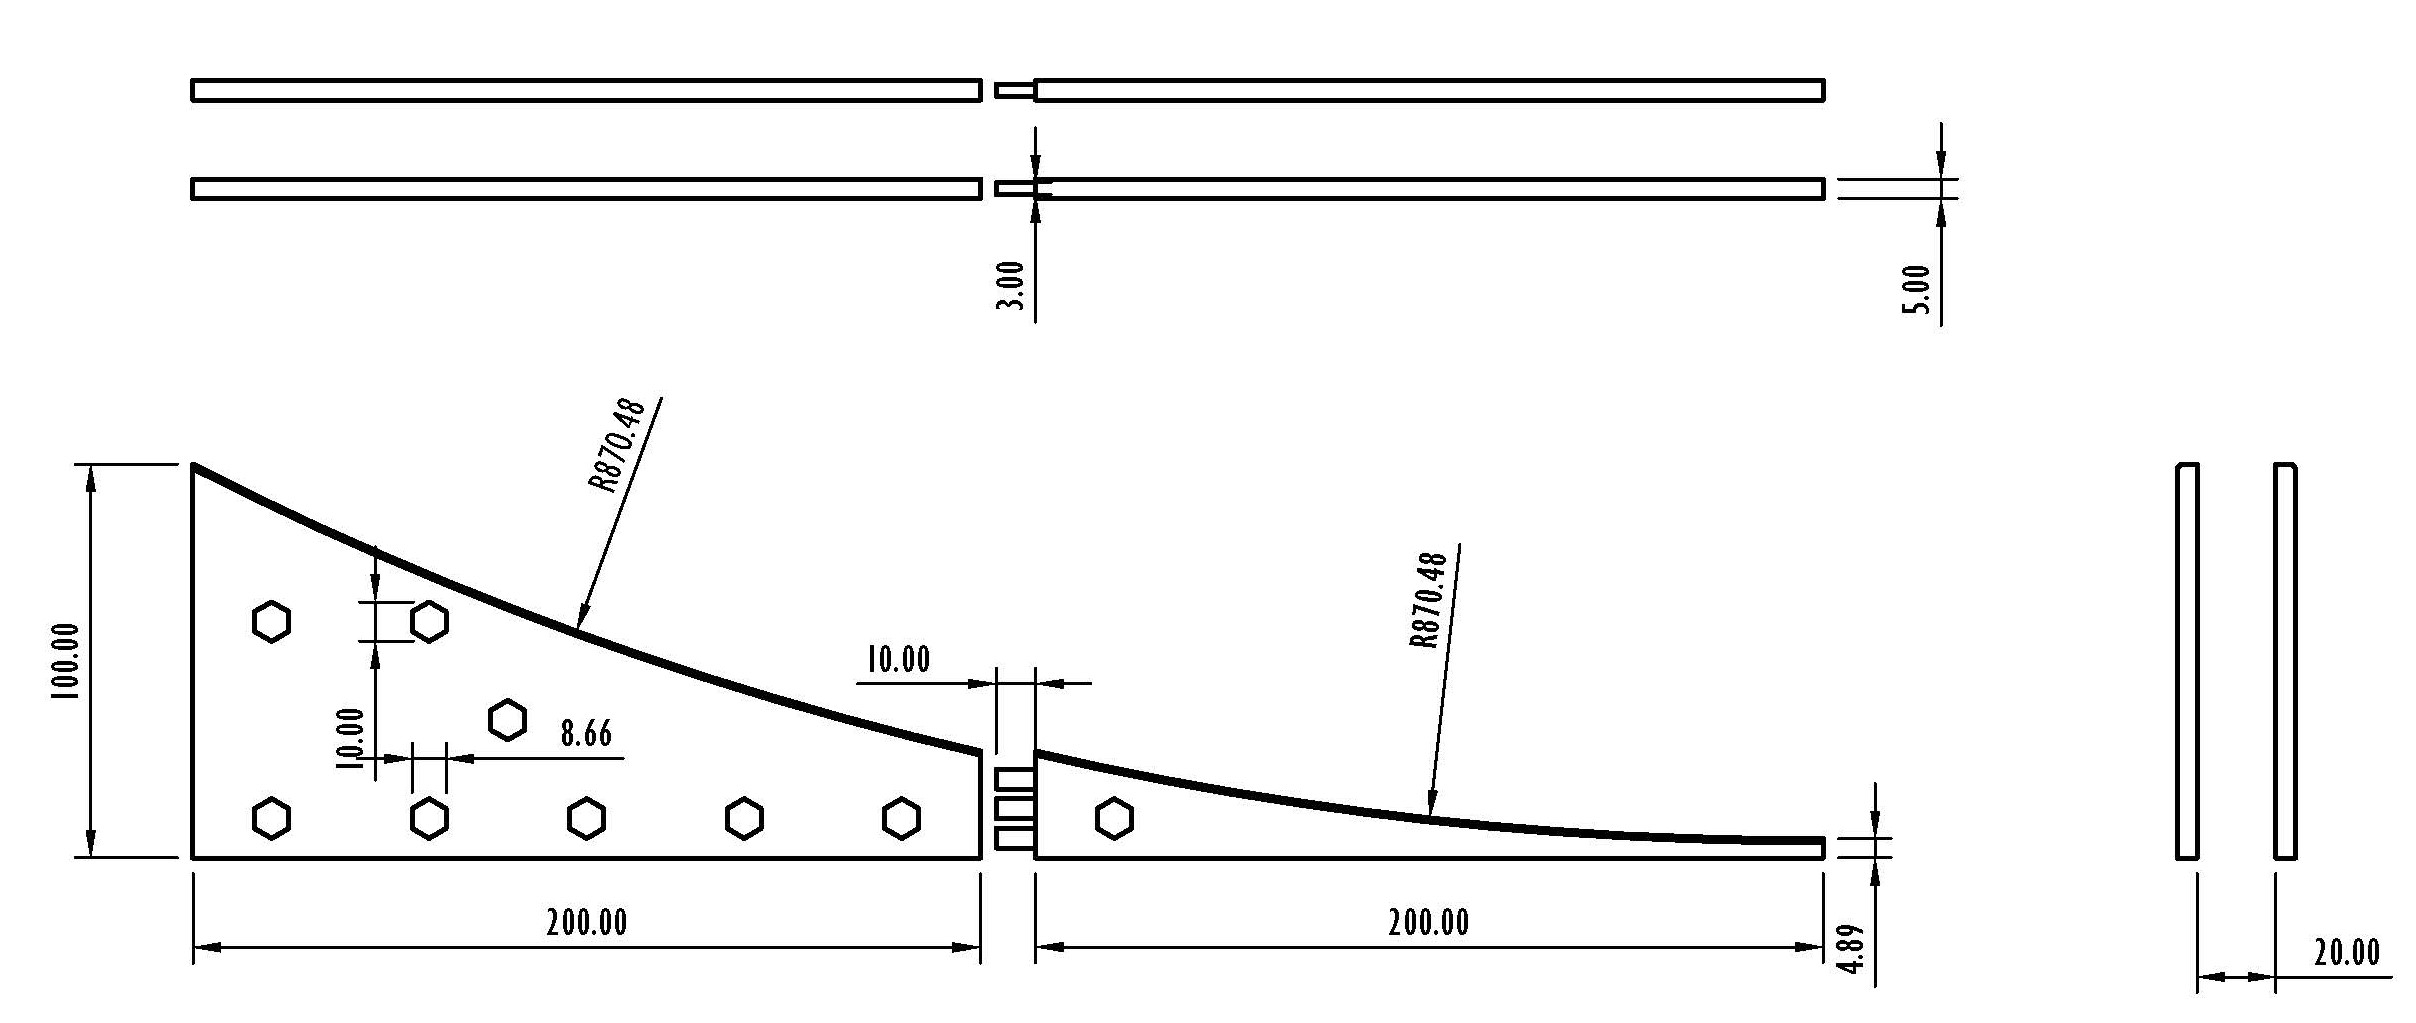
\includegraphics[width=0.99\textwidth]{images/rampedraw2.jpg}
  \caption[Technische Zeichnung der Beschleunigereinheit]{Zu sehen ist eine technische Zeichnung der geplanten Beschleunigereinheit, die auf einen 3D-Druck ausgelegt ist, jedoch mit leichten Anpassungen auch auf einer \textsw{CNC-Fräse} aus einer Stahlplatte mit Dicke $d=\SI{5}{\milli\metre}$ gefertigt werden kann. Die Rampe besitzt durch  die Aussparung eines Kreisbogens mit Radius $r=\SI{900}{\milli\metre}$ von $\SI{267.2}{\degree}$ bis $\SI{270}{\degree}$ einen nahezu waagerechten Auslauf.}
  \label{fig:rampedraw}
  \vspace{-0pt}
\end{figure}

\noindent Die Schiene dieser Rampe ist zweigeteilt und hat jeweils eine Aussägung in Form eines Kreisbogens mit Radius $r=\SI{900}{\milli\metre}$ von $\SI{267.2}{\degree}$ bis $\SI{270}{\degree}$. Die sechseckigen Aussparungen sind für die Aufnahme von Muttern gedacht, die mittels \textit{WIG}-Schweißen (\textsw{W}olfram-\textsw{I}nert\textsw{g}as) befestigt werden können. Oben links an der Vorderseite wird eine rechtsdrehende, auf der Rückseite eine linksdrehende Mutter verwendet. Die Mutterorientierung muss sich immer abwechseln, damit angebrachte Zahnräder gleichgerichtet drehen. Durch die mechanische Werkstatt werden Gewindestangen geschnitten, die jeweils hälftig aus Links- und Rechtsgewinde bestehen. 

An diese Gewindestangen werden einseitig die Zahnräder mit \textit{Madenschrauben} befestigt. Somit kann die Rampe bei Drehung des linken oberen Zahnrades nach rechts zusammen und bei Drehung nach links auseinander gefahren werden.

Da die Rampe möglichst schnell funktionsfähig sein muss, und gewisse Probleme mit dem vorhandenem 3D-Drucker bestehen, wird die Rampe aus Sperrholz selbst angefertigt, wie auf Foto \ref{fig:rampenschliff1} zu sehen ist. Die Aussparungen für die Muttern --- welche anschließend eingeklebt werden --- entstehen durch Bearbeitung mit einem Stechbeitel der Eisenbreite $\SI{3}{\milli\metre}$. Die Muttern werden anschließend eingeklebt und die beiden Rampensegmente mit den Gewindestangen verbunden.

%% Autor: Björn Ritterbecks 
%% Letzte Aenderung: 15.06.2016 
\thisfloatsetup{%
  capbesidewidth=\marginparwidth}
\begin{figure}[htbp]
\centering
%\sansmath
 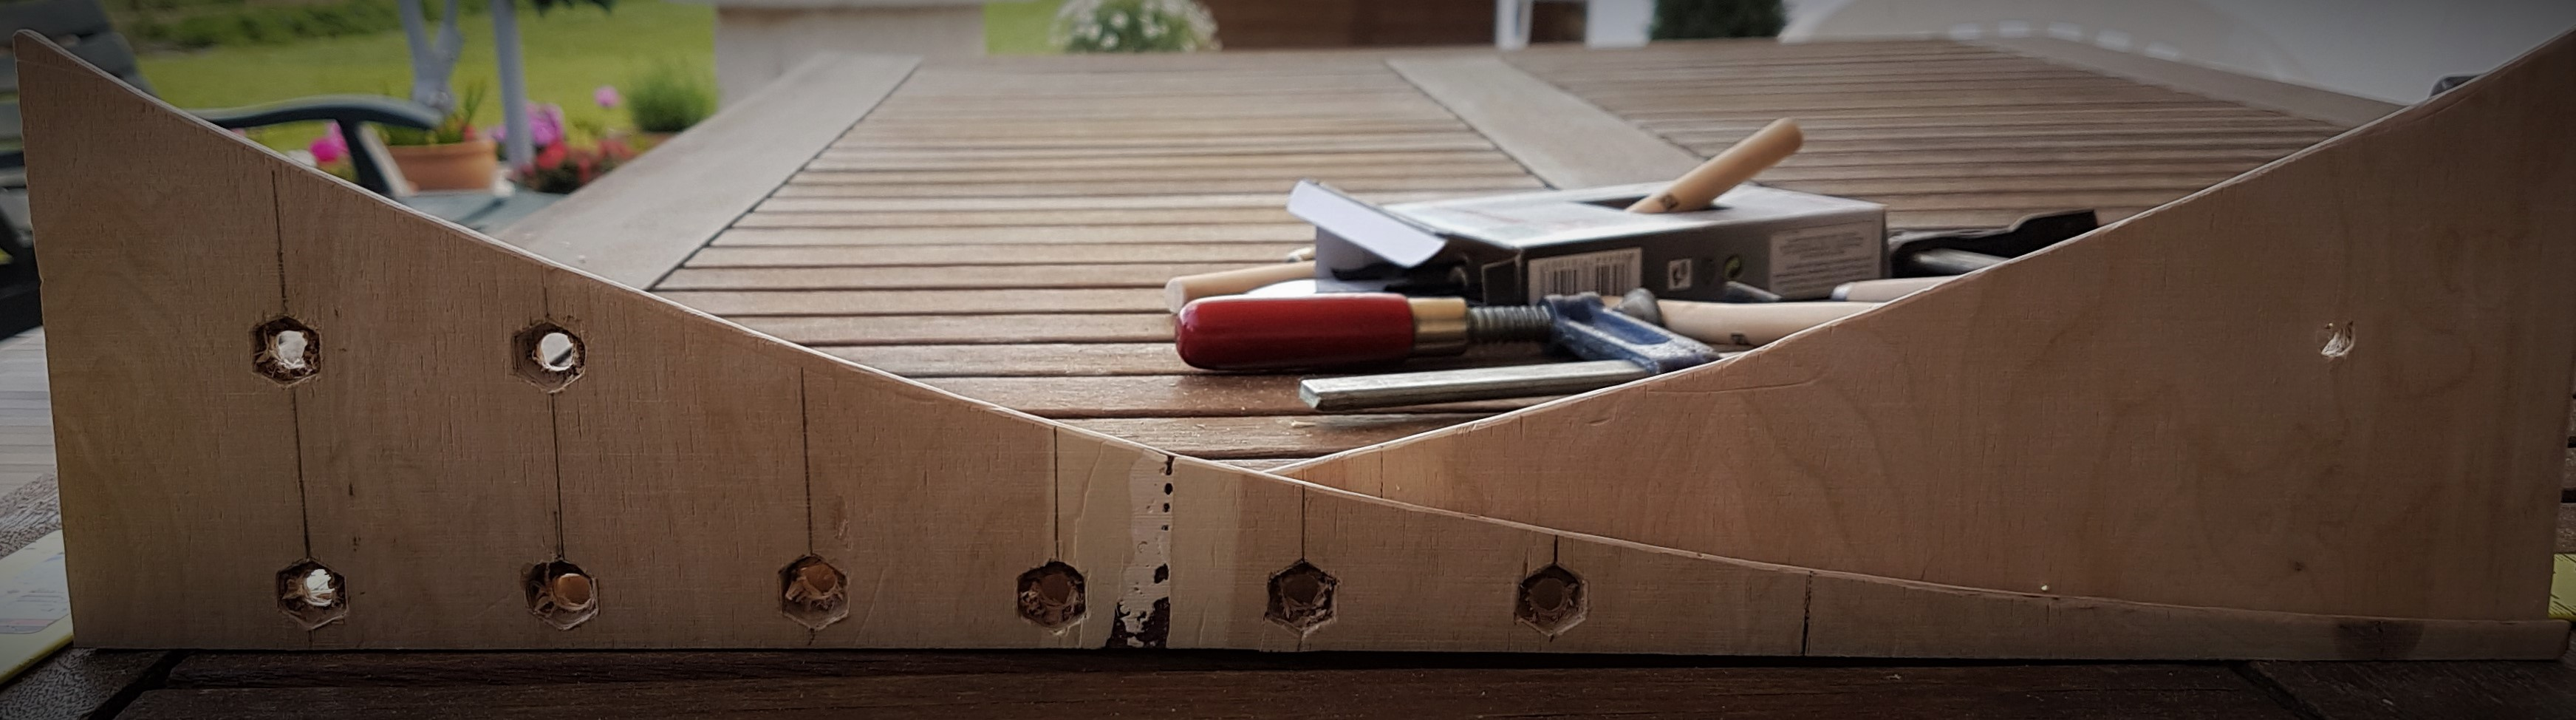
\includegraphics[width=0.99\textwidth]{images/rampenschliff1.jpg}
  \caption[Gesägte und gehobelte Rampensegmente]{Seitenansicht der gebauten Rampensegmente. Mittels eines nicht dehnbaren Fadens, Winkeln und einigen Schraubzwingen wird die Form angezeichnet und anschließend auf der Abfallseite ausgesägt. Die Annäherung an die endgültige Form erfolgt durch einen fein eingestellten Schweifhobel. Nach dem Durchbohren mit einem $\SI{6}{\milli\metre}$ Bohrer werden die Aussparungen für die Mutteraufnahme mit einem Stechbeitel gefertigt.}
  \label{fig:rampenschliff1}
  \vspace{-0pt}
\end{figure}

\noindent Bei der Arbeit mit Holz ist eine Genauigkeit von einem halben Millimeter bereits ordentlich, die von der Werkstatt --- aus Aluminium --- geschnittenen Gewinde verzeihen jedoch kaum ein Abweichen von der Parallelität der Muttern. Da Aluminium ein weicher Werkstoff mit hohem Abrieb ist, sind die Gewinde schnell zerstört. Bei einem erneuten Bau sollten sie demnach zumindest aus Messing gefertigt werden.

%% Autor: Björn Ritterbecks 
%% Letzte Aenderung: 15.06.2016 
\thisfloatsetup{%
  capbesidewidth=\marginparwidth}
\begin{figure}[htbp]
\vspace*{0.2cm}
\centering
%\sansmath
 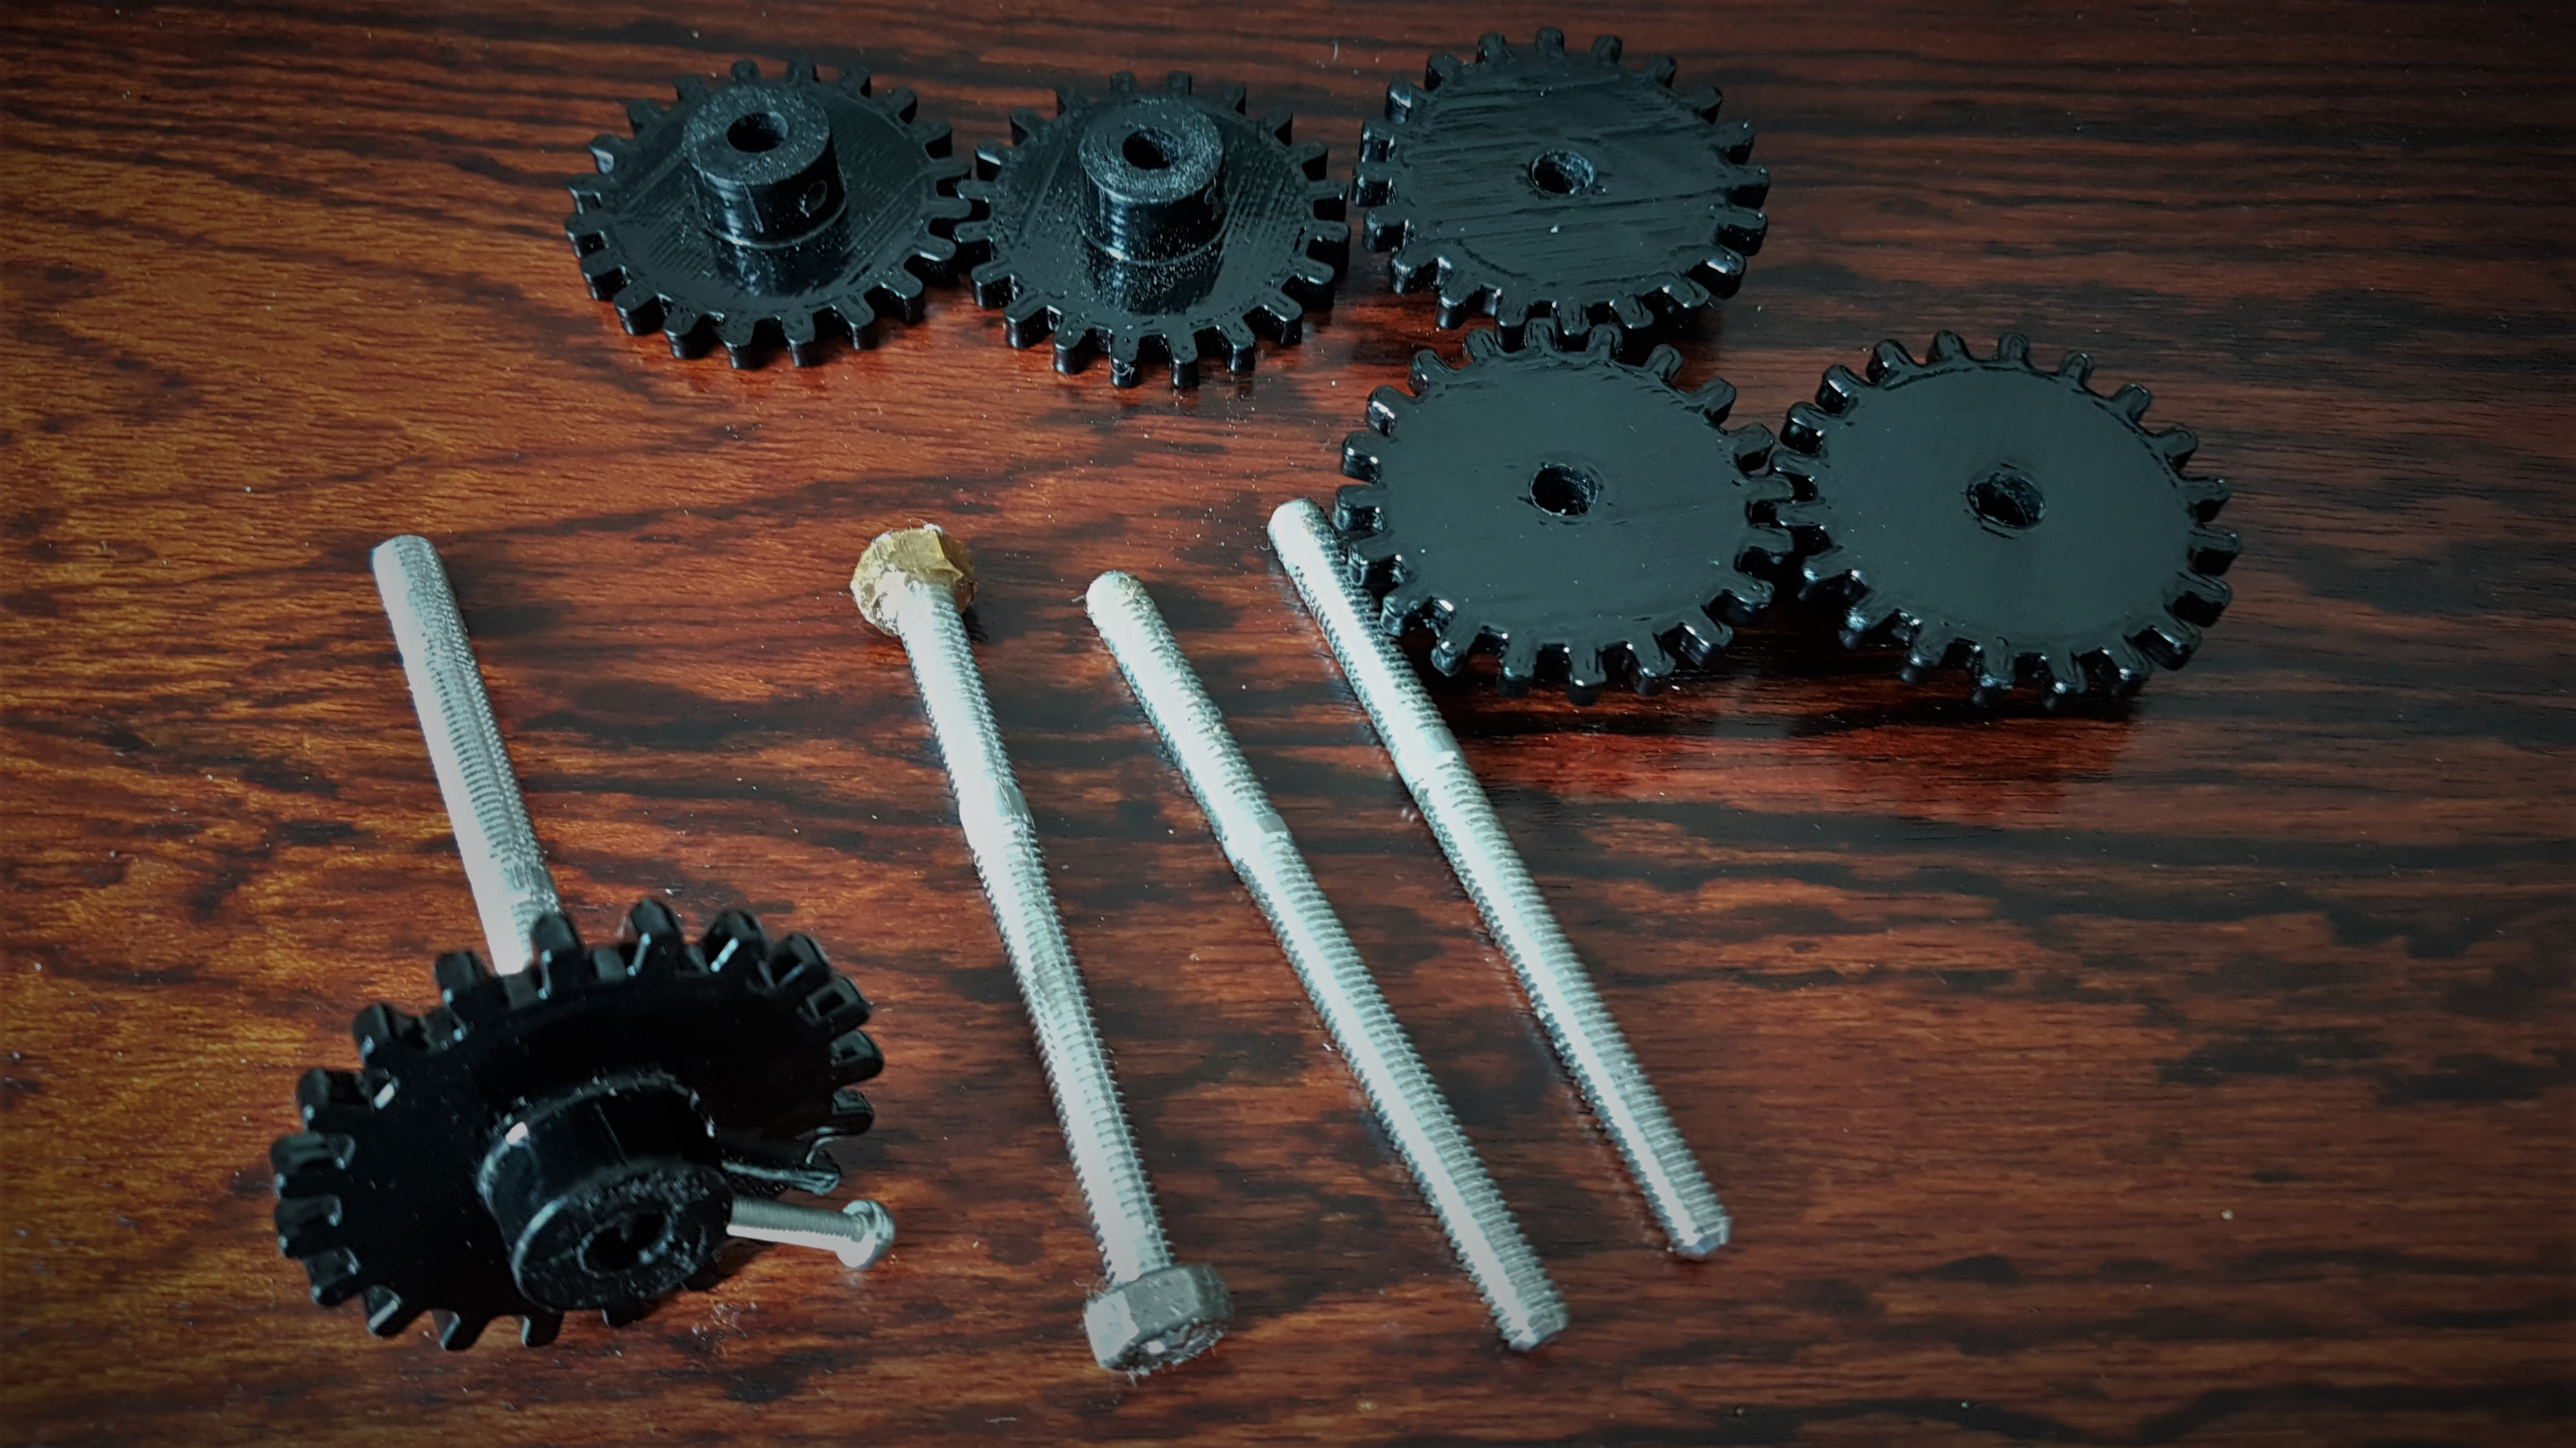
\includegraphics[width=0.99\textwidth]{images/toothpaste.jpg}
  \caption[Fotografie der Zahnräder und Gewinde]{Fotografische Abbildung der Zahnräder und Gewinde nach dem Ausbau. Bei Versuchen vor dem Einkleben der Muttern haben beide Komponenten gut funktioniert, wurden jedoch bei der Arretierung an der Beschleunigereinheit in ihrer Funktionalität zerstört (unter anderem durch Kleberückstände und mangelhafte Parallelität).}
  \label{fig:toothpaste}
  \vspace{-0pt}
\end{figure}

Die Zahnräder werden mit dem 3D-Drucker bei maximaler Dichte aus \textit{ABS} (\textsw{A}crylnitril-\textsw{B}utadien-\textsw{S}tyrol) gedruckt, um das Schneiden eines Gewindes für die Madenschrauben zu ermöglichen. Anschließend werden Ungenauigkeiten des Druckergebnisses in einem \textit{Aceton-Dampfbad} bereinigt. Sowohl die Zahnräder als auch die Gewinde sind in Abbildung \ref{fig:toothpaste} dargestellt. Problematisch ist jedoch, dass die Gewinde schon bei recht geringem Zug ausreißen, da der verwendete Kunststoff nicht hart genug ist.

Trotz der Unwägsamkeiten wird die Rampe mit der Vorrichtung aus Abbildung \ref{fig:rampfenschliff2} an den Experimentiertisch geschraubt. Eine Kugel wird auf das waagerechte Rampensegment gelegt, welches so auseinander-/zusammengeschoben wird, bis die Kugel die Tischplatte leicht berührt. Der Aufbau ist trotz der fehlenden Automatisierung praktikabel, wenn beide Gleise einzeln justiert und mit Gewindestangen fixiert werden.

%% Autor: Björn Ritterbecks 
%% Letzte Aenderung: 15.06.2016 
\thisfloatsetup{%
  capbesidewidth=\marginparwidth}
\begin{figure}[htbp]
\vspace*{0.2cm}
\centering
%\sansmath
 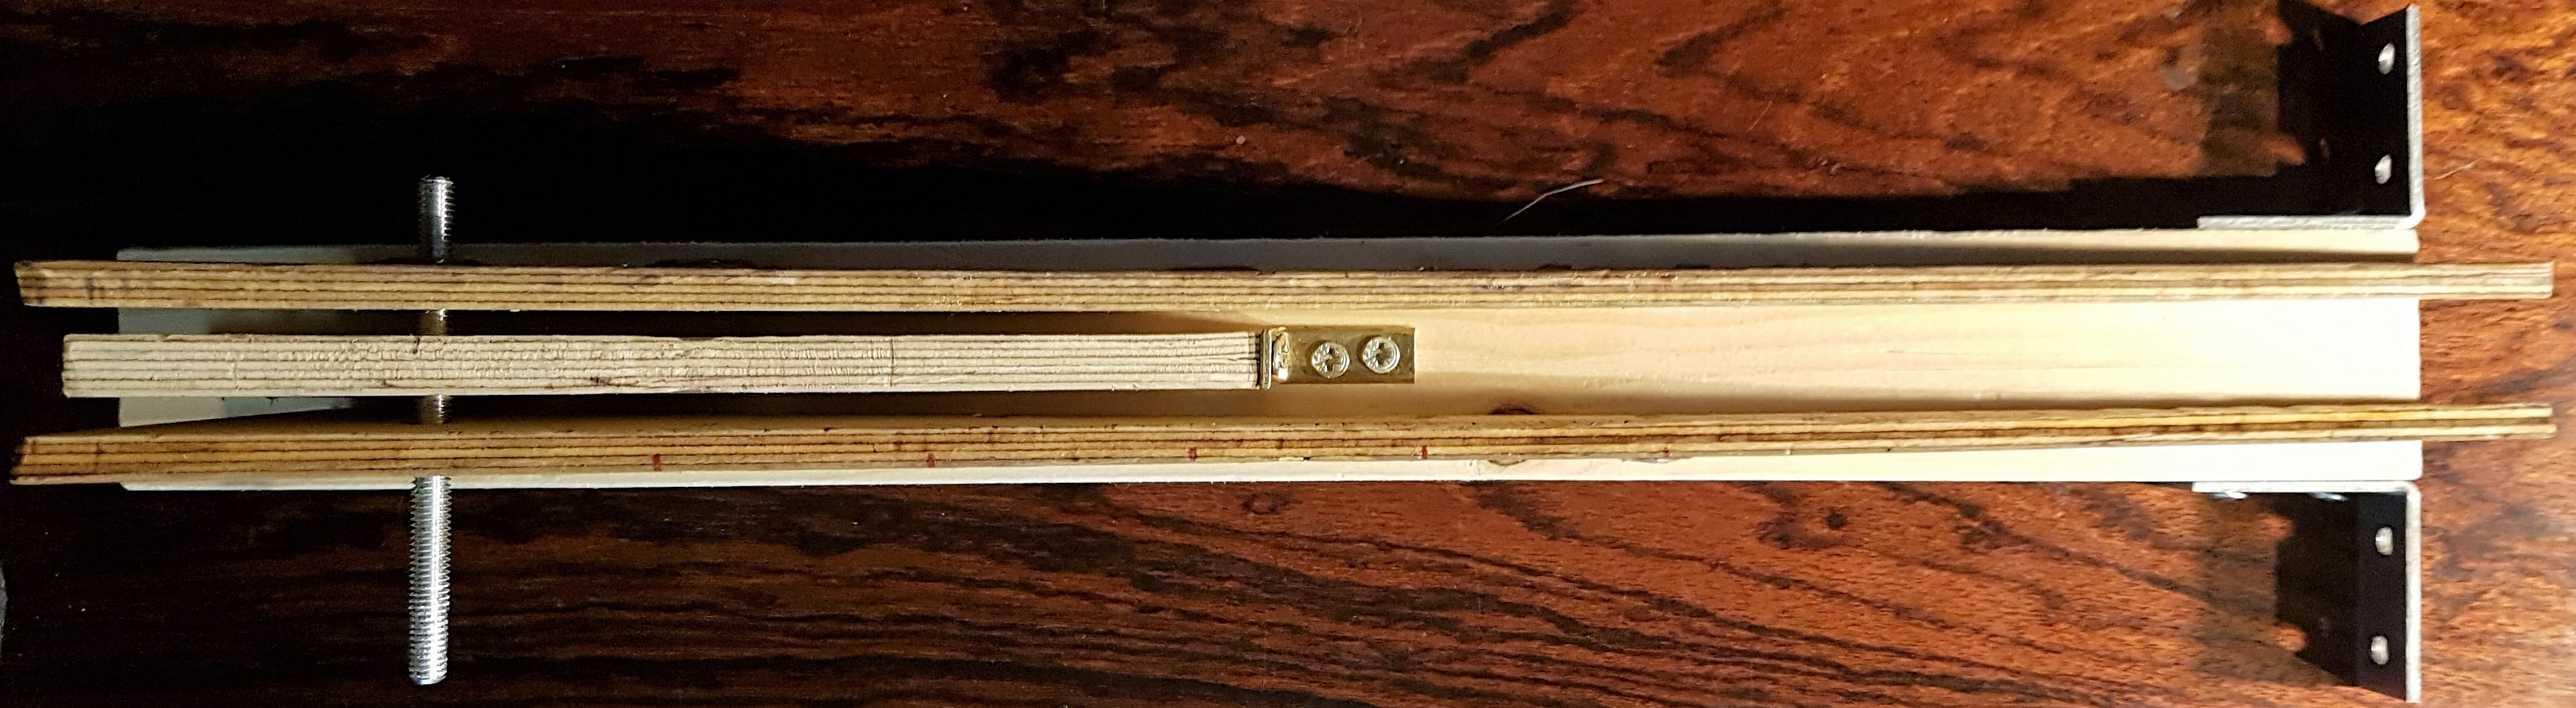
\includegraphics[width=0.99\textwidth]{images/rrampe1.jpg}
  \caption[Draufsicht der gebauten Rampe]{Die Startrampe ist auf ein Brett montiert, welches wiederum mit zwei Winkeln an den Experimentiertisch angeschraubt werden kann. Durch die Anordnung auf einem schmalen Brett lässt sich zum Einen die Rechtwinkligkeit gut überprüfen, zum Anderen erlaubt es den Zahnrädern in vertikaler Richtung bis unterhalb der Tischplatte zu reichen. Auf der linken Seite mittig ist ein Holzblock mit Ausbohrungen, durch welche die Gewindestangen zur Zentrierung gesteckt hätten werden sollen.}
  \label{fig:rampfenschliff2}
  \vspace{-0pt}
\end{figure}

\section{Kugeln}
\label{sec:balls}

Wie in den Analogiebetrachtungen bereits erwähnt, gibt es zwei Anforderungen an die Ionenanalogie: Es werden Kugeln benötigt, die in ihrer Größe und Dichte unterscheidbar sind. Um die Analogie $\sfrac{q}{m}\widehat{=}\sfrac{A_\mathrm{proj}}{m}$ weiter zu verbessern, soll die Quantelung der Ladung berücksichtigt werden, indem $A_{\mathrm{proj},i}=i\cdot A_{\mathrm{proj},0}$ gilt. Dies wäre zum Beispiel bei den Kugelradien $\SI{10}{\milli\metre}$, $\SI{14}{\milli\metre}$, $\SI{17}{\milli\metre}$ und $\SI{20}{\milli\metre}$ näherungsweise erfüllt.

Da frei verfügbare Kugeln meistens in einer Schrittweite von $\SI{5}{\milli\metre}$ zu kaufen sind, entfällt diese Möglichkeit. Eine Anfrage an Produzenten von Präzisionskugeln verschiedener Werkstoffe ergab für einen Satz von 4 Kugelradien und 4 Werkstoffen gut unterscheidbarer Dichte, d.\,h. 160 Kugeln, einen Preis über $1\,000,-\euro$. 

Eine weitere Möglichkeit, diese Forderungen zu erfüllen, wird darin gesehen, einen 3D-Drucker zu verwenden und die Füllung zwar homogen, jedoch zwischen den einzelnen Kugelarten unterscheidbar zu gestalten (bei 3D-Druckern besteht die Möglichkeit, die Dichte des Füllmaterials zu bestimmen). 

%% Autor: Björn Ritterbecks 
%% Letzte Aenderung: 15.06.2016 
\thisfloatsetup{%
  capbesidewidth=\marginparwidth}
\begin{figure}[htbp]
\centering
%\sansmath
 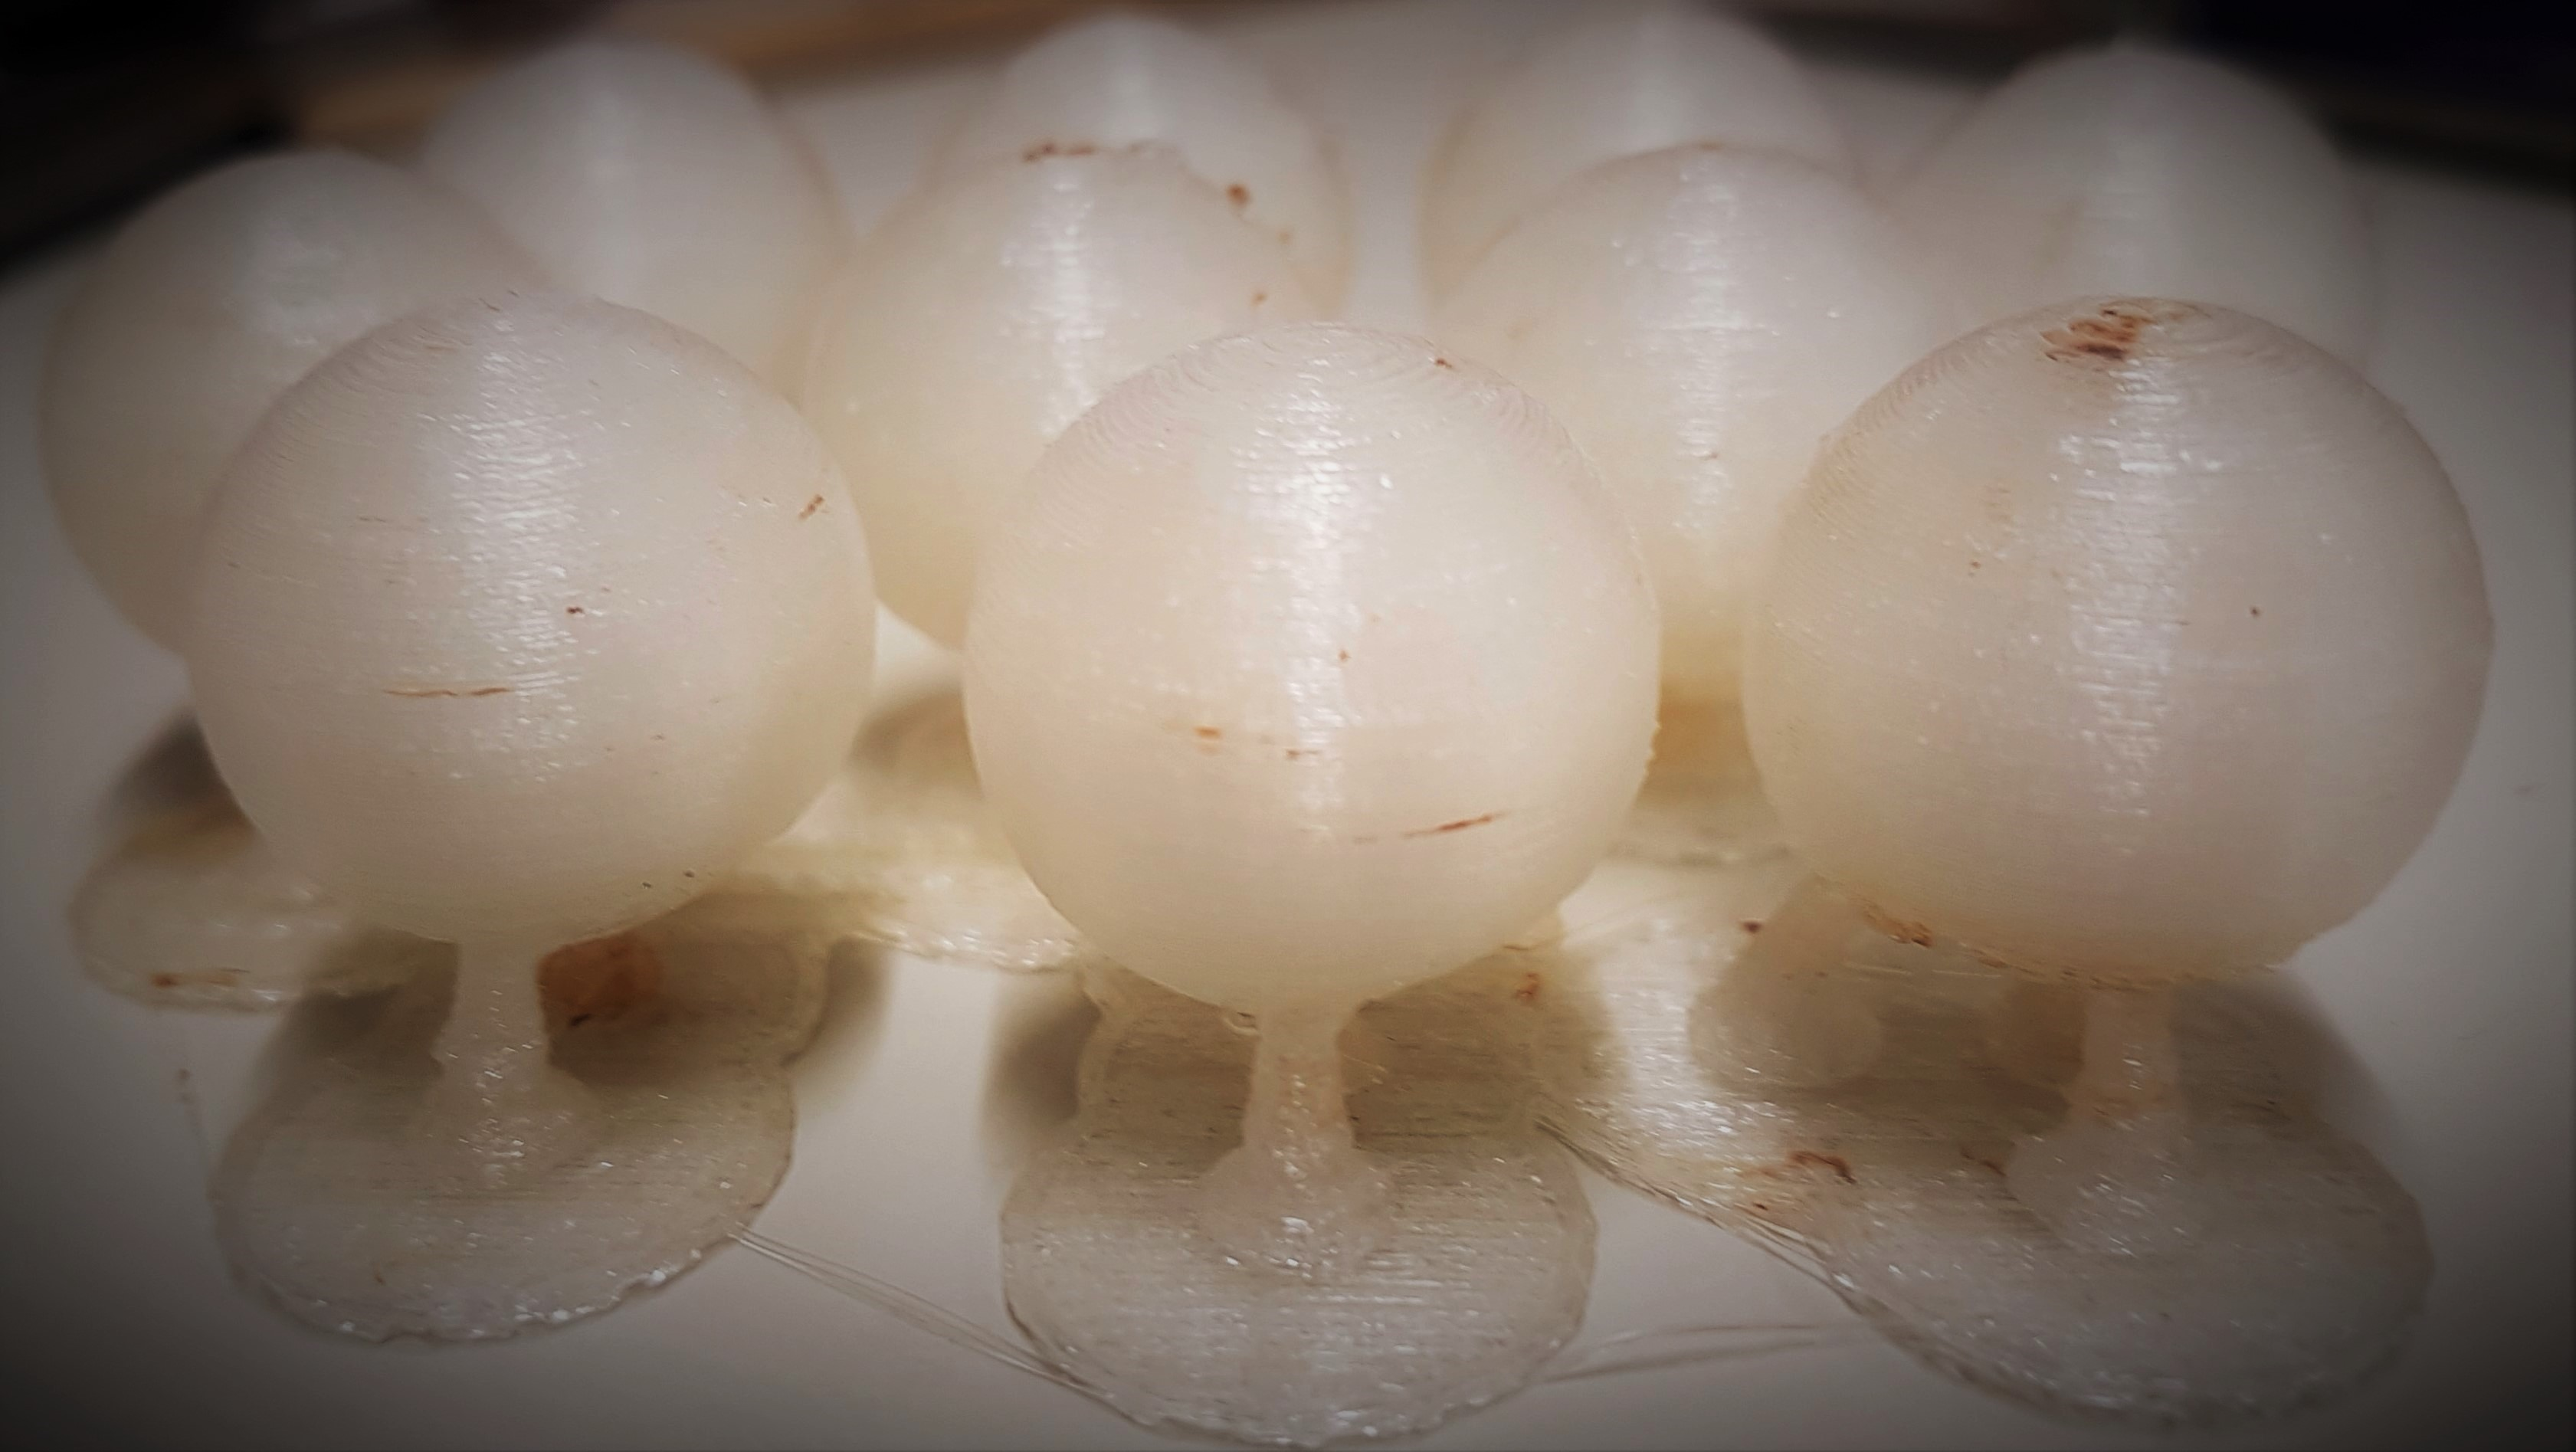
\includegraphics[width=0.99\textwidth]{images/gedrucktekugeln2.jpg}
  \caption[3D-gedruckte Kugeln]{Zu sehen ist der erste Versuch für 3D-gedruckte Kugeln auf einem Stützensystem.}
  \label{fig:gedrucktekugeln2}
  \vspace{-0pt}
\end{figure}

\noindent Nach einem Probedruck von zwei Kugelhälften, die jeweils auf der Flachen Seite erstellt worden sind, wird der erste Satz von 10 Kugeln mit maximaler Dichte und einem Radius von $\SI{10.0}{\milli\metre}$ auf einem Stelzengeflecht gedruckt (siehe Abb. \ref{fig:gedrucktekugeln2}). Dieser Druck ergibt leider kein gutes Resultat, da die Unterseiten abgeflacht und somit die Kugeln nicht Rotationssymmetrisch sind. Bei dem Versuch, jeweils zwei Kugelhälften mit Aceton zusammenzukleben, fiel jedoch, wie auf Foto \ref{fig:fail} zu sehen ist, auf, dass trotz maximaler Druckdichte die Kugelschale wesentlich dichter gedruckt ist, als das Innenleben, und somit keine homogene Massenverteilung gewährleistet wird. 

%% Autor: Björn Ritterbecks 
%% Letzte Aenderung: 15.06.2016 
\thisfloatsetup{%
  capbesidewidth=\marginparwidth}
\begin{figure}[htbp]
\vspace*{0.2cm}
\centering
%\sansmath
 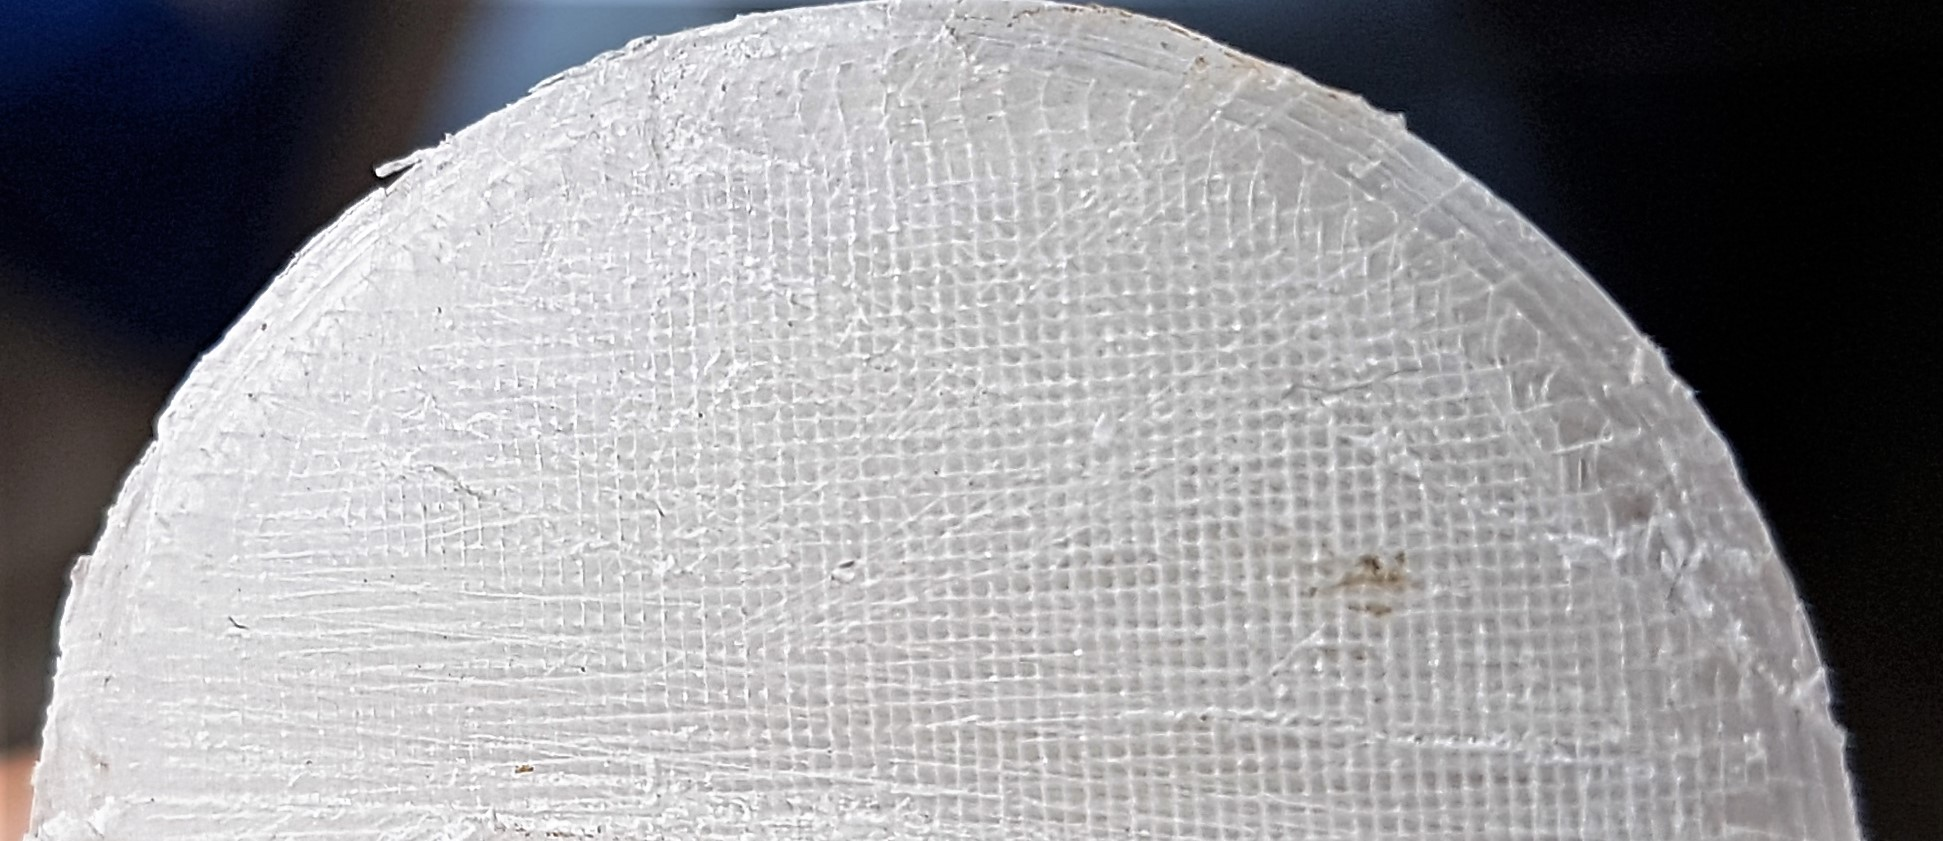
\includegraphics[width=0.99\textwidth]{images/fail.jpg}
  \caption[Aufgeschnittene Kugel aus dem 3D-Drucker]{Auf diesem Foto einer aufgeschnittenen, 3D-gedruckten Kugel ist gut zu erkennen, dass die Wandschicht der Kugel mit einer höheren Dichte gedruckt wurde.}
  \label{fig:fail}
  \vspace{-0pt}
\end{figure}

\noindent Um dennoch die restlichen Komponenten zufriedenstellend untersuchen zu können, wurden im Anschluss Holzkugeln aus dem Bastelbedarf und Glaskugeln (einfache Murmeln) gekauft. 

\section{Schiefe Ebene}

Die erste Hälfte der Experimentierplatte zu einer schiefen Ebene zu machen, während die zweite Hälfte in der Waage bleibt, wird realisiert, indem beide Teilplatten separat auf jeweils vier Standfüße, die unabhängig voneinander einstellbar sind, montiert werden, so dass beim Aneinanderschieben der beiden Platten die rechte waagerecht ist und die linke Platte an der Vorderkante einige Millimeter höher und an der Hinterkante dieselbe Distanz tiefer, jedoch in $x$-Richtung ebenfalls in der Waage liegt.

Die Fixierung der beiden Platten und damit auch die Möglichkeit eines Transportes wird durch gehobelte Bretter umgesetzt, bei denen jeweils eine Hälfte um einige Zehntelmillimeter abgeschrägt wird, während die andere Hälfte um die festgelegte Anzahl an Millimetern abgeschabt wird (siehe Foto \ref{fig:brettvorderplatte}). Auf diese Weise kann die Neigung der schiefen Ebene festgelegt werden. Beispielsweise bei einer Plattenbreite von $\SI{40}{\centi\metre}$ führen jeweils $\SI{2}{\milli\metre}$ an der Vorder- und Hinterkante zu einer Neigung von $1:100$.

%% Autor: Björn Ritterbecks 
%% Letzte Aenderung: 15.06.2016 
\thisfloatsetup{%
  capbesidewidth=\marginparwidth}
\begin{figure}[htbp]
\vspace*{0.2cm}
\centering
%\sansmath
 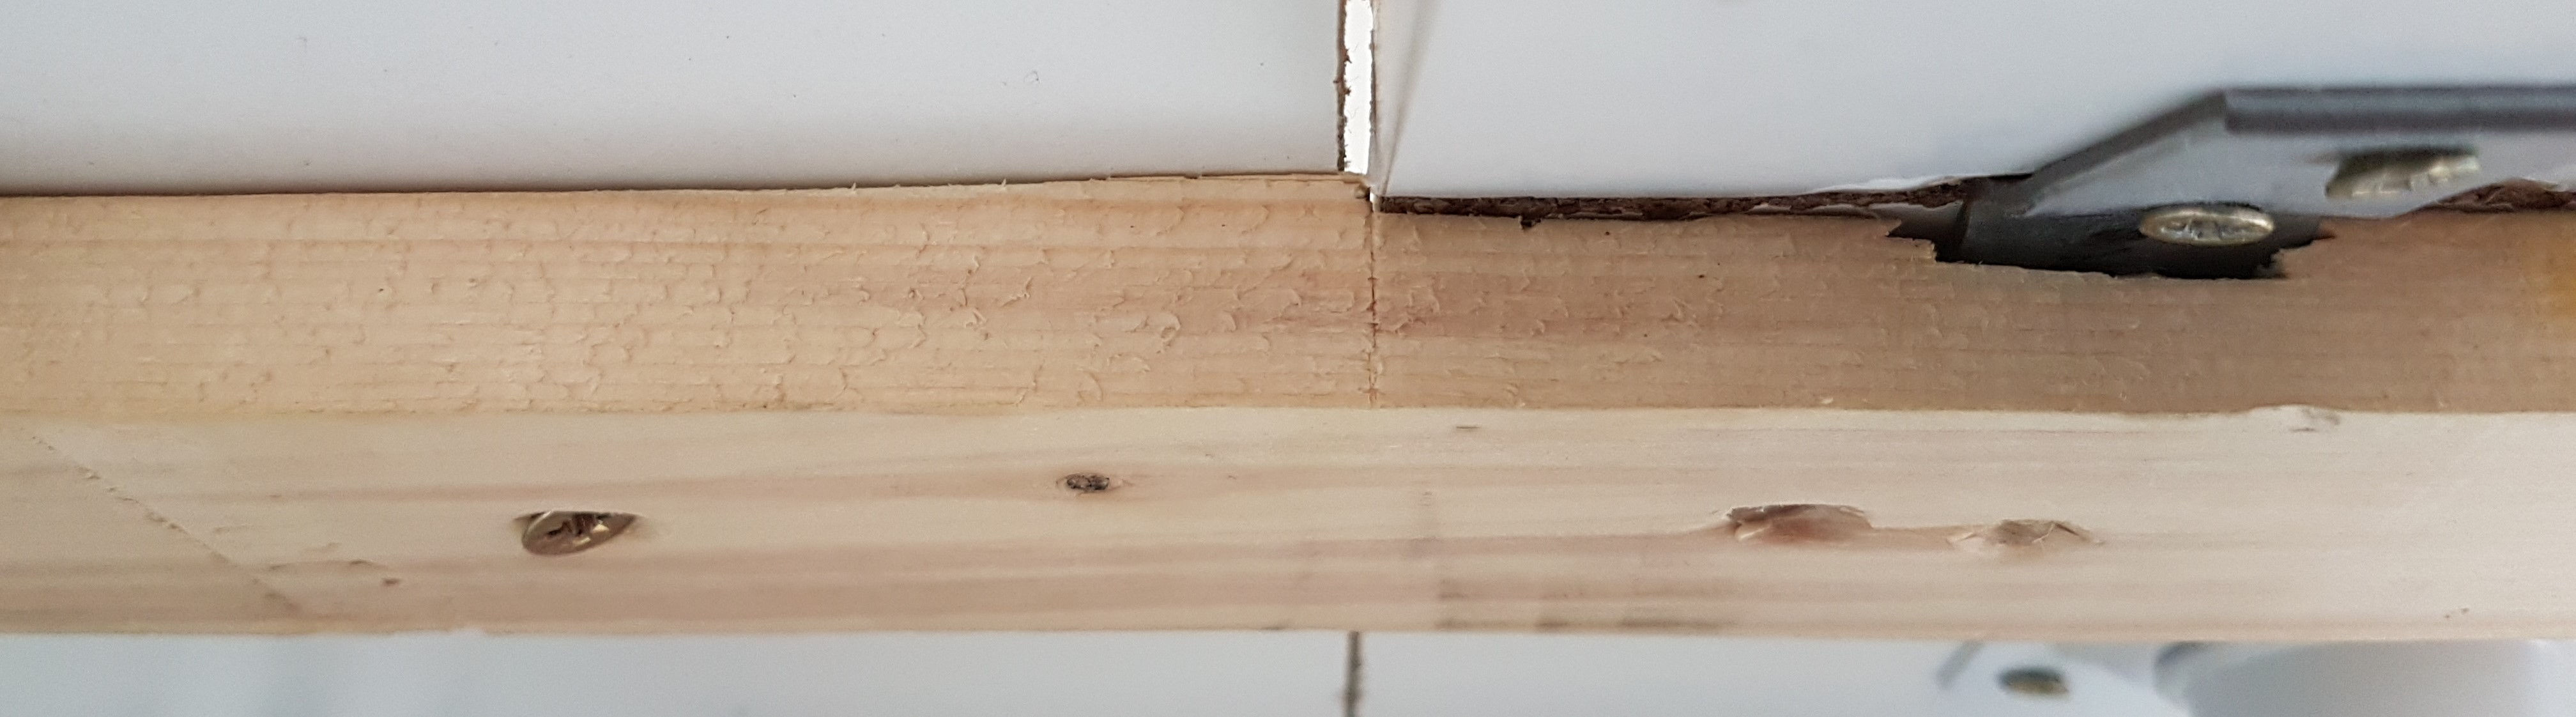
\includegraphics[width=0.99\textwidth]{images/brettvorderplatte.jpg}
  \caption[Übergangsbereich schiefe Ebene]{Zu sehen ist der Übergangsbereich zwischen schiefer Ebene und waagerechter Platte, der jeweils an der Vorder- und Hinterkante mit einem passend abgehobeltem Brett fixiert wird. Der um $\SI{15}{\degree}$ geneigte Plattenteil ist erst nach den Messungen hinzugefügt worden, um der Winkelaufspaltung der Kugeln genüge zu tun (d.\,h., dass die Breiten der einzelnen Detektoren nach rechts hin zunehmen müssen.)}
  \label{fig:brettvorderplatte}
  \vspace{-0pt}
\end{figure}

\noindent Im Übergangsbereich der Platten wird --- wie bei \textcite{Schilling1987} --- Isolierband geklebt, damit die Kugeln den Höhenunterschied möglichst ohne Aufprallen/Springen überwinden können. Die Festlegung der Plattenneigung erfolgt über Berechnungen in \textit{Excel} und beträgt bei den Messungen ca. $1:35$, da eine möglichst große Auslenkung auf der schiefen Ebene gewünscht ist. Wie die Messungen zeigen werden, sollte jedoch für den endgültigen Aufbau ein geringeres Gefälle gewählt werden. Der Baustand während der Probemessungen kann in Abbildung \ref{fig:aufbau1} betrachtet werden.

%% Autor: Björn Ritterbecks 
%% Letzte Aenderung: 15.06.2016 
\thisfloatsetup{%
  capbesidewidth=\marginparwidth}
\begin{figure}[htbp]
\vspace*{0.2cm}
\centering
%\sansmath
 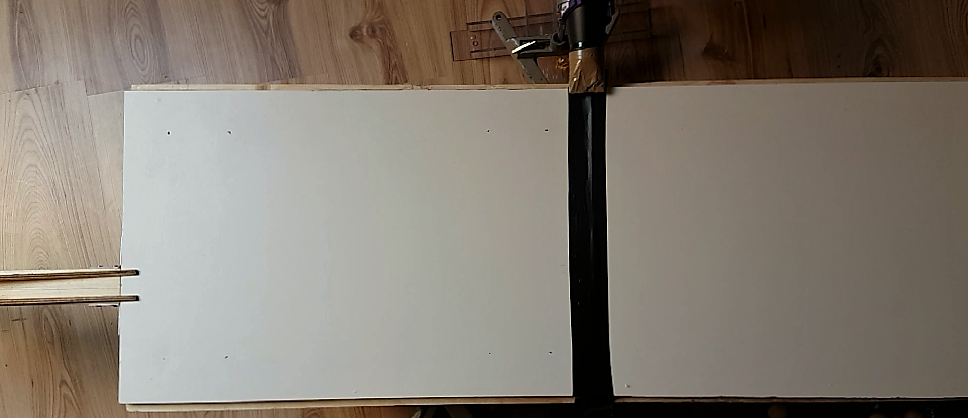
\includegraphics[width=0.99\textwidth]{images/Aufbau.png}
  \caption[Versuchsaufbau ohne Detektoren]{Fotografie des Versuchsaufbaus ohne Detektoren. Bei der linken Platte handelt es sich um die schiefe Ebene. Das Gebläse wirkt mit der höchsten Kraft im Übergangsbereich der beiden Platten. Durch die Aufhängung mit Winkeln kann die Rampe auch näher am Gebläse positioniert werden.}
  \label{fig:aufbau1}
  \vspace{-0pt}
\end{figure}

\section{Detektoren}



Wie bereits von \textsc{Mais} angemerkt, geschieht die Aufspaltung der analysierten Teilchen (Kugeln) radialsymmetrisch um den Punkt der größten Krafteinwirkung. Auch bei einem geschwindigkeitsfokussierenden Aufbau ändert sich nichts an diesem Prinzip, wobei jedoch zwischen den langsamsten und schnellsten Kugeln ein mittlerer Auslenkwinkel bestimmt werden muss. Aufgrund der Unzulänglichkeiten der verwendeten Holz- und Glaskugeln ist diese Kalibrierung noch nicht erfolgen.
An dieser Stelle wird dennoch der Versuch unternommen, die Grundlagen einer praktischen Umsetzung zu beschreiben.
%% Autor: Björn Ritterbecks 
%% Letzte Aenderung: 15.06.2016 
\begin{marginfigure}
\vspace*{0.2cm}
\centering
%\sansmath
 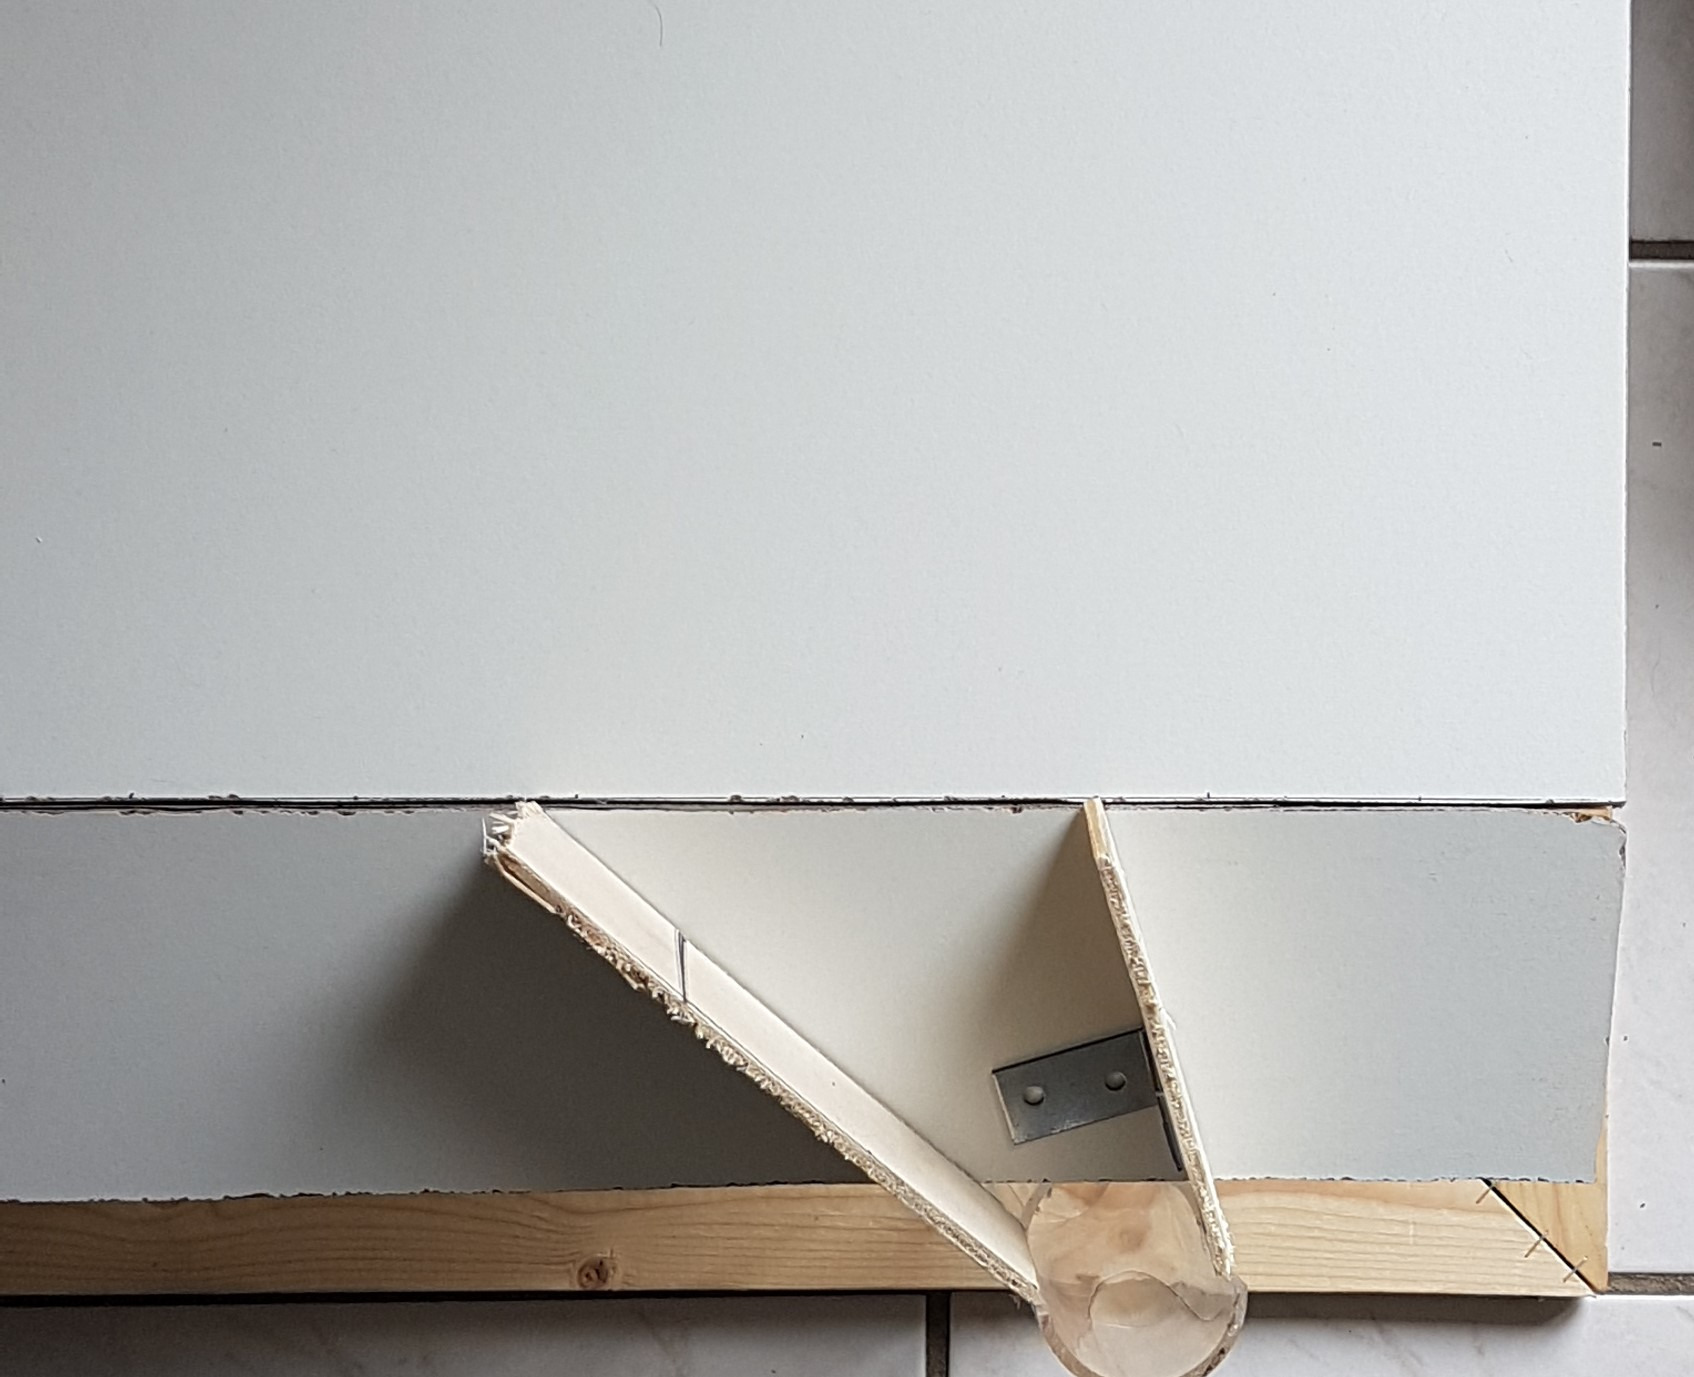
\includegraphics[width=0.99\marginparwidth]{images/istregistriert.jpg}
  \caption[Detektionsnsprinzip]{Vorschlag einer Detektoranordnung: Je geringer der Detektionswinkel ist, desto größer muss die Breite der einzelnen Detektoren sein. Damit selbst bei den größten Detektoren alle Kugeln in die Röhren rollen können, ist der rechte Teil der Platte um $\SI{15}{\degree}$ geneigt. Ein letzter Detektor wird am rechten Ende angebracht.}
  \label{fig:istregisrtiert}
  \vspace{-0pt}
\end{marginfigure}

Bei dem Aufbau nach \textcite{Schilling1987} sind die Detektoren in einem festen Abstand $b$ zueinander angebracht. Dies führt allerdings --- bereits bei oberflächlicher Betrachtung dazu, dass ein Teil der weiter rechts liegenden Detektoren nur noch einige $\SI{E-1}{\degree}$ detektieren kann. Die waagerechte Platte ist ca. $\SI{65}{\centi\metre}$ lang, die schiefe Ebene etwa $\SI{55}{\centi\metre}$ (vgl. \ref{fig:mnu}). Somit entspricht die Ablenkung im Gravitationsfeld bei einer Starthöhe von $\SI{2}{\centi\metre}$ bis $\SI{8}{\centi\metre}$ zwischen $\SI{5}{\centi\metre}$ und $\SI{1}{\centi\metre}$. Nimmt man an, dass bei \textsc{Schilling} jeder Detektor eine Breite von $\SI{9}{\centi\metre}$ hat, so würde der letzte Detektor in einem Winkel zwischen $\SI{5.5}{\degree}$ und $\SI{4.7}{\degree}$ getroffen werden (bei den langsamsten Kugeln) und zwischen $\SI{1.2}{\degree}$ und $\SI{1.0}{\degree}$ bei den schnellsten, jedoch der erste Detektor bei den langsamen Kugeln im Bereich von $\SI{90}{\degree}$ bis $\SI{39}{\degree}$.

Diese qualitativen Rechnungen gelten natürlich nur, wenn die Detektion auf der Fokussierungsachse erfolgen soll. Da die Impulsänderung $\Delta p$ linear mit dem Gewicht skaliert, wird schnell klar, dass im Bereich hoher Kugeldichten der Analysator ein hohes Auflösungsvermögen hätte, wenn die Analysatorlänge stark ausgedehnt werden würde. 

Damit wird eine L-förmige Detektoranordnung vorgeschlagen, die auch Massen mit einem Registrierwinkel nahe $\SI{1}{\degree}$ wahrnehmen kann. Die Konzeption ist auf dem Foto \ref{fig:istregisrtiert} zu sehen: Je schwerer die Massen sind, desto weiter rechts werden sie detektiert und umso geringer ist der Auftreffwinkel. Somit bräuchten die linken Detektoren keine Breitenanpassung, sondern erst diejenigen weiter rechts. Da die Kugeln bei einem geringen Auftreffwinkel an den Begrenzungen der Detektoren hängen bleiben könnten, wird die waagerechte Platte bei $y=0$ abgetrennt und mit einer Neigung von $\SI{15}{\degree}$ erneut angeschraubt. Dieses Prinzip ist bereits 1970 in ähnlicher Form von der \textsc{Nuffield Foundation} verwendet worden (vgl. Abb. \ref{fig:nuffsaid}).


